% Options for packages loaded elsewhere
\PassOptionsToPackage{unicode}{hyperref}
\PassOptionsToPackage{hyphens}{url}
%
\documentclass[
]{book}
\usepackage{lmodern}
\usepackage{amsmath}
\usepackage{ifxetex,ifluatex}
\ifnum 0\ifxetex 1\fi\ifluatex 1\fi=0 % if pdftex
  \usepackage[T1]{fontenc}
  \usepackage[utf8]{inputenc}
  \usepackage{textcomp} % provide euro and other symbols
  \usepackage{amssymb}
\else % if luatex or xetex
  \usepackage{unicode-math}
  \defaultfontfeatures{Scale=MatchLowercase}
  \defaultfontfeatures[\rmfamily]{Ligatures=TeX,Scale=1}
\fi
% Use upquote if available, for straight quotes in verbatim environments
\IfFileExists{upquote.sty}{\usepackage{upquote}}{}
\IfFileExists{microtype.sty}{% use microtype if available
  \usepackage[]{microtype}
  \UseMicrotypeSet[protrusion]{basicmath} % disable protrusion for tt fonts
}{}
\makeatletter
\@ifundefined{KOMAClassName}{% if non-KOMA class
  \IfFileExists{parskip.sty}{%
    \usepackage{parskip}
  }{% else
    \setlength{\parindent}{0pt}
    \setlength{\parskip}{6pt plus 2pt minus 1pt}}
}{% if KOMA class
  \KOMAoptions{parskip=half}}
\makeatother
\usepackage{xcolor}
\IfFileExists{xurl.sty}{\usepackage{xurl}}{} % add URL line breaks if available
\IfFileExists{bookmark.sty}{\usepackage{bookmark}}{\usepackage{hyperref}}
\hypersetup{
  pdftitle={Network Medicine},
  pdfauthor={Deisy Morselli Gysi},
  hidelinks,
  pdfcreator={LaTeX via pandoc}}
\urlstyle{same} % disable monospaced font for URLs
\usepackage{color}
\usepackage{fancyvrb}
\newcommand{\VerbBar}{|}
\newcommand{\VERB}{\Verb[commandchars=\\\{\}]}
\DefineVerbatimEnvironment{Highlighting}{Verbatim}{commandchars=\\\{\}}
% Add ',fontsize=\small' for more characters per line
\usepackage{framed}
\definecolor{shadecolor}{RGB}{248,248,248}
\newenvironment{Shaded}{\begin{snugshade}}{\end{snugshade}}
\newcommand{\AlertTok}[1]{\textcolor[rgb]{0.94,0.16,0.16}{#1}}
\newcommand{\AnnotationTok}[1]{\textcolor[rgb]{0.56,0.35,0.01}{\textbf{\textit{#1}}}}
\newcommand{\AttributeTok}[1]{\textcolor[rgb]{0.77,0.63,0.00}{#1}}
\newcommand{\BaseNTok}[1]{\textcolor[rgb]{0.00,0.00,0.81}{#1}}
\newcommand{\BuiltInTok}[1]{#1}
\newcommand{\CharTok}[1]{\textcolor[rgb]{0.31,0.60,0.02}{#1}}
\newcommand{\CommentTok}[1]{\textcolor[rgb]{0.56,0.35,0.01}{\textit{#1}}}
\newcommand{\CommentVarTok}[1]{\textcolor[rgb]{0.56,0.35,0.01}{\textbf{\textit{#1}}}}
\newcommand{\ConstantTok}[1]{\textcolor[rgb]{0.00,0.00,0.00}{#1}}
\newcommand{\ControlFlowTok}[1]{\textcolor[rgb]{0.13,0.29,0.53}{\textbf{#1}}}
\newcommand{\DataTypeTok}[1]{\textcolor[rgb]{0.13,0.29,0.53}{#1}}
\newcommand{\DecValTok}[1]{\textcolor[rgb]{0.00,0.00,0.81}{#1}}
\newcommand{\DocumentationTok}[1]{\textcolor[rgb]{0.56,0.35,0.01}{\textbf{\textit{#1}}}}
\newcommand{\ErrorTok}[1]{\textcolor[rgb]{0.64,0.00,0.00}{\textbf{#1}}}
\newcommand{\ExtensionTok}[1]{#1}
\newcommand{\FloatTok}[1]{\textcolor[rgb]{0.00,0.00,0.81}{#1}}
\newcommand{\FunctionTok}[1]{\textcolor[rgb]{0.00,0.00,0.00}{#1}}
\newcommand{\ImportTok}[1]{#1}
\newcommand{\InformationTok}[1]{\textcolor[rgb]{0.56,0.35,0.01}{\textbf{\textit{#1}}}}
\newcommand{\KeywordTok}[1]{\textcolor[rgb]{0.13,0.29,0.53}{\textbf{#1}}}
\newcommand{\NormalTok}[1]{#1}
\newcommand{\OperatorTok}[1]{\textcolor[rgb]{0.81,0.36,0.00}{\textbf{#1}}}
\newcommand{\OtherTok}[1]{\textcolor[rgb]{0.56,0.35,0.01}{#1}}
\newcommand{\PreprocessorTok}[1]{\textcolor[rgb]{0.56,0.35,0.01}{\textit{#1}}}
\newcommand{\RegionMarkerTok}[1]{#1}
\newcommand{\SpecialCharTok}[1]{\textcolor[rgb]{0.00,0.00,0.00}{#1}}
\newcommand{\SpecialStringTok}[1]{\textcolor[rgb]{0.31,0.60,0.02}{#1}}
\newcommand{\StringTok}[1]{\textcolor[rgb]{0.31,0.60,0.02}{#1}}
\newcommand{\VariableTok}[1]{\textcolor[rgb]{0.00,0.00,0.00}{#1}}
\newcommand{\VerbatimStringTok}[1]{\textcolor[rgb]{0.31,0.60,0.02}{#1}}
\newcommand{\WarningTok}[1]{\textcolor[rgb]{0.56,0.35,0.01}{\textbf{\textit{#1}}}}
\usepackage{longtable,booktabs}
\usepackage{calc} % for calculating minipage widths
% Correct order of tables after \paragraph or \subparagraph
\usepackage{etoolbox}
\makeatletter
\patchcmd\longtable{\par}{\if@noskipsec\mbox{}\fi\par}{}{}
\makeatother
% Allow footnotes in longtable head/foot
\IfFileExists{footnotehyper.sty}{\usepackage{footnotehyper}}{\usepackage{footnote}}
\makesavenoteenv{longtable}
\usepackage{graphicx}
\makeatletter
\def\maxwidth{\ifdim\Gin@nat@width>\linewidth\linewidth\else\Gin@nat@width\fi}
\def\maxheight{\ifdim\Gin@nat@height>\textheight\textheight\else\Gin@nat@height\fi}
\makeatother
% Scale images if necessary, so that they will not overflow the page
% margins by default, and it is still possible to overwrite the defaults
% using explicit options in \includegraphics[width, height, ...]{}
\setkeys{Gin}{width=\maxwidth,height=\maxheight,keepaspectratio}
% Set default figure placement to htbp
\makeatletter
\def\fps@figure{htbp}
\makeatother
\setlength{\emergencystretch}{3em} % prevent overfull lines
\providecommand{\tightlist}{%
  \setlength{\itemsep}{0pt}\setlength{\parskip}{0pt}}
\setcounter{secnumdepth}{5}
\usepackage{booktabs}
\usepackage{DejaVuSans}
\usepackage[left=1in, right=1in, bottom=1in, top=1in]{geometry}
\usepackage{hyperref}
\ifluatex
  \usepackage{selnolig}  % disable illegal ligatures
\fi
\usepackage[]{natbib}
\bibliographystyle{apalike}

\title{Network Medicine}
\author{Deisy Morselli Gysi}
\date{2021-02-03}

\begin{document}
\maketitle

{
\setcounter{tocdepth}{1}
\tableofcontents
}
\hypertarget{workshop-on-network-medicine}{%
\chapter{Workshop on Network Medicine}\label{workshop-on-network-medicine}}

Network medicine (\textbf{NetMed}) is a field of Network Science that uses Systems Biology to understand its impact on medicine, and it is mostly focused on network topology. In NetMed we often use biological networks to represent the topological space and it be used to identify disease modules, their relationship to other diseases, drug repurpusing, and drug combinations. The biological networks often used for it are based on protein-protein interactions (PPI), Gene-Disease-Associations (GDA), and Drug-Targets.

In this workshop, we will learn:

\begin{itemize}
\tightlist
\item
  how to identify disease modules (Session \ref{diseasemodule});
\item
  how to predict disease comorbidities (Session \ref{dissep});
\item
  how to repurpuse drugs using a network approach (Session \ref{proximity}).
\end{itemize}

\hypertarget{whatarenets}{%
\section{What are networks?}\label{whatarenets}}

\begin{quote}
Adapted from \citet{Gysi2020}.
\end{quote}

Network Science is broadly employed in many fields: from understanding \emph{how friends bond in a party} to \emph{how animals interact}; from \emph{how superheroes appear in the same comic books} to \emph{how genes can be related to a specific biological process}. Network analysis is especially beneficial for understanding complex systems, in all research fields. Examples of complex biological or medical systems include gene regulatory, ecological and neuropsychology networks. In this workshop, focus is given to applications of Network Science to the medical sciences.

Here, I will start by introducing the basic network terminologies and then explore how can we define and identify disease modules, identify disease commorbidities and lastly, we will learn how to repurpuse drugs for diseases with known modules. For each step, I will then present some classical and some new studies.

It is expected some degree of familiarity with \texttt{R}, \texttt{ggplot2}, \texttt{tidyr}, and \texttt{igraph}.

\hypertarget{terminology}{%
\section{Terminology}\label{terminology}}

While the nature of each system, i.e.~what its entities are and what kind of interactions they have, is different, there are common notations. A short review of common network terms can be found in Session \ref{network-terminology} and a brief review of biological terms can be found in Session \ref{biological-terminology}.

The set of interactions among a set of entities is, in general, called a graph or a network \citep{Newman2018, Barabasi2016}. In graph theory, each entity is called a vertex, while in network notation it is called a node \citep{Barabasi2016}. Accordingly, the connections between two entities are called edges or links, respectively \citep{Barabasi2016}. In this workshop, I will always use the network notation, unless otherwise specified. The total number of nodes in a network is often denoted as \textbf{N} and the number of links in a network is denoted as \textbf{L}. While nodes can receive a label, links in general, are not labeled \citep{Barabasi2016} (although, in many cases, weights can also be perceived as a label). A network can be represented mathematically as an adjacency matrix (usually denoted as \textbf{A}) (Table \ref{tab:ADJ}), an edge-list (Table \ref{tab:EL}), or visually as a graph (Figure \ref{fig:GRAPH}).

\begin{table}

\caption{\label{tab:ADJ}Mathematical Representation of a Network: Adjacency Matrix}
\centering
\begin{tabular}[t]{l|r|r|r|r|r|r|r|r|r|r}
\hline
  & A & C & B & D & H & F & J & I & E & G\\
\hline
A & 0 & 1 & 1 & 1 & 0 & 0 & 0 & 1 & 1 & 0\\
\hline
C & 1 & 0 & 0 & 0 & 1 & 0 & 1 & 0 & 0 & 0\\
\hline
B & 1 & 0 & 0 & 1 & 0 & 1 & 0 & 0 & 0 & 1\\
\hline
D & 1 & 0 & 1 & 0 & 0 & 0 & 0 & 0 & 0 & 0\\
\hline
H & 0 & 1 & 0 & 0 & 0 & 0 & 0 & 0 & 0 & 0\\
\hline
F & 0 & 0 & 1 & 0 & 0 & 0 & 0 & 0 & 0 & 0\\
\hline
J & 0 & 1 & 0 & 0 & 0 & 0 & 0 & 0 & 0 & 0\\
\hline
I & 1 & 0 & 0 & 0 & 0 & 0 & 0 & 0 & 0 & 0\\
\hline
E & 1 & 0 & 0 & 0 & 0 & 0 & 0 & 0 & 0 & 0\\
\hline
G & 0 & 0 & 1 & 0 & 0 & 0 & 0 & 0 & 0 & 0\\
\hline
\end{tabular}
\end{table}

Links of a network can possess a direction (normally depicted by an arrow), which indicates that the interaction is asymmetric, e.g.~one gene is regulating another gene, or a person follows somebody else in a social network. Networks with directed links are called directed networks, while networks without directed interactions or in which the direction is not known are referred to as undirected networks, e.g.~collaboration in the same study or interactions between proteins. In NetMed - and in this workshop - most of the times we assume that networks do not posses a direction. The links can also have a weight to express the strength of the interaction, which results in a weighted network \citep{Newman2018, Barabasi2016}. Usually, the weight is graphically displayed as the thickness or the length of the links.

\begin{table}

\caption{\label{tab:EL}Mathematical Representation of a Network: Edge List}
\centering
\begin{tabular}[t]{l|l}
\hline
Source & Target\\
\hline
A & D\\
\hline
C & H\\
\hline
B & F\\
\hline
C & J\\
\hline
A & I\\
\hline
B & D\\
\hline
A & B\\
\hline
A & E\\
\hline
B & G\\
\hline
A & C\\
\hline
\end{tabular}
\end{table}

Networks can also have different dimensions. These dimensions can be understood as layers (or different link types) of the same system \citep{Kurant2006LayeredNetworks, Kivela2014MultilayerNetworks}. For example, in a multi-omics multilayer system, each layer can be constructed using different -omics data (for example genomics, transcriptomics, proteomics, etc.) where the `whole' biological system can be understood as a network of networks \citep{DeDomenico2017}. The topology and the dynamic properties of the whole network can be changed by simply transforming the weights of the interactions, or by ignoring that nodes can interact in many ways \citep{Mucha2010CommunityNetworks, Radicchi2013AbruptNetworks} also ignoring the node's importance to the system. We will not deal with multi-layer networks in this workshop.

\begin{figure}

{\centering 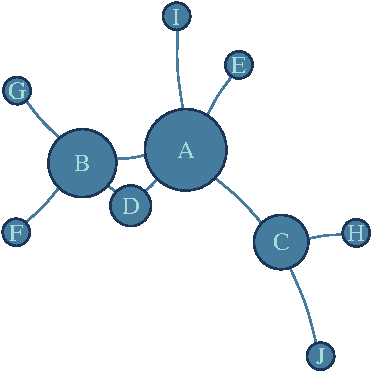
\includegraphics[width=0.8\linewidth]{NetMed_files/figure-latex/GRAPH-1} 

}

\caption{Visual Representation of a Network: Graph}\label{fig:GRAPH}
\end{figure}

\hypertarget{network-terminology}{%
\subsection{Network Terminology}\label{network-terminology}}

\begin{itemize}
\item
  A \textbf{network} is a pair \textbf{G = (N, L)} of a set \textbf{N} of nodes connected by a set \textbf{L} of links.
\item
  Two nodes are \textbf{neighbours} if they are \textbf{connected}. The \textbf{degree} (d) of a node is the \textbf{number of nodes} it interacts with \citep{Bondy2008GraphTheory}.
\item
  The \textbf{weight} is a measure of how strong a particular interaction is \citep{Bondy2008GraphTheory}.
\item
  The \textbf{strength} of a node is the \textbf{sum of the weights} attached to links belonging to a node \citep{Barrat2003TheNetworks}.
\item
  The \textbf{direction} of a link specifies the source (starting point) and a target (endpoint) where the interaction occurs \citep{Barabasi2016} .
\item
  \textbf{Hubs} are nodes with a \textbf{much larger degree} compared to the average degree value \citep{Barrat2003TheNetworks}.
\item
  A set of highly interconnected nodes is a \textbf{module} or \textbf{cluster} \citep{Li2009}. Two nodes are connected in a network, if a sequence of adjacent nodes, a \textbf{path}, connects them \citep{barabasi2004network}.
\item
  The \textbf{shortest path length} is the number of links along the shortest path connecting two nodes \citep{barabasi2004network}.
\item
  The \textbf{average path length} is the average of the shortest paths between all pairs of nodes \citep{barabasi2004network}.
\item
  The \textbf{diameter} is the maximum distance between two nodes \citep{Bondy2008GraphTheory}.
\item
  The \textbf{modularity index} is a measure of the strength of the network division into modules when this measure is maximized; it can be used for identifying nodes communities \citep{Newman2018}.
\item
  \textbf{Preferential attachment} is the tendency of nodes to form new links preferentially to nodes with a high number of links \citep{barabasi1999emergence, Vazquez2003GrowingCorrelations}.
\item
  The probability that a random node in the network has a particular degree is given by the \textbf{degree distribution} \citep{barabasi2004network}.
\item
  A \textbf{bipartide graph} is a network in which the nodes can be divided into two disjoint sets of nodes such that links connect nodes from the two sets to each other, but never inside the same set \citep{Barabasi2016}. In those networks, most of the network measures are calculated differently than in a unipartide network.
\item
  The \textbf{clustering coefficient} describes the degree with which a node is connected to all its neighbours \citep{barabasi2004network}.
\item
  The \textbf{global clustering} coefficient measures the total number of triangles in a network \citep{Barabasi2016}.
\item
  The \textbf{average clustering} coefficient is the average of the clustering coefficient of all nodes in a network \citep{barabasi2004network}.
\item
  \textbf{Centrality} is a set of measures that have been proposed to help to define the most central nodes. It has many interpretations for autonomy, control, risk, exposure, influence and power \citep{Borgatti2006ACentrality}.

  \begin{itemize}
  \item
    \textbf{Closeness centrality} is defined as the average distance from a single vertex to all other vertices\citep{Newman2018}.
  \item
    \textbf{Betweenness centrality} is defined as the total number of shortest paths between pairs of nodes that pass through a particular node \citep{Newman2018}.
  \end{itemize}
\item
  \textbf{Global measures} are measures that describe the whole network, for example, \emph{degree distribution; average clustering coefficient; path length; modularity index}.
\item
  \textbf{Local measures} are characteristics of individual nodes of a network, such as their \emph{degree} and \emph{centrality}.
\end{itemize}

\hypertarget{biological-terminology}{%
\subsection{Biological Terminology}\label{biological-terminology}}

\begin{itemize}
\item
  \textbf{DNA} is the hereditary material of most organisms -- usually all cells of an organism have the same DNA \citep{Slack2013}.
\item
  \textbf{Genes} are the basic physical and functional units of heredity. They are parts of the DNA and contain the information for producing functional RNAs and proteins. \citep{Slack2013}.
\item
  \textbf{Proteins} are large, complex molecules that play many critical roles in the body. The proteins are responsible for most of the work in cells and are necessary for structure, function, and regulation of the cells. They can act as enzymes, antibodies, transporters, transcription factors etc. \citep{Slack2013}.
\item
  The \textbf{RNA} is synthesized from the DNA but has different properties and functions than the DNA. Some RNAs carry out biological functions in a cell, while others, messenger RNA (mRNA), are turned into proteins that fulfil biological functions \citep{Slack2013}.
\item
  A \textbf{non-coding RNA (ncRNA)} is an RNA that does not encode a protein. NcRNAs often play a role in gene regulation \citep{MattickNon-codingRNA}.
\item
  \textbf{microRNAs (miRNA)} are examples of ncRNA; they are involved in posttranscriptional regulation of protein expression \citep{Tanase2012MicroRNAs}.
\item
  \textbf{Gene expression} is, in short, the coupled process of transcription (from DNA to RNA) and translation (from RNA to proteins) to transform the stored information inside the DNA into proteins \citep{Slack2013}.
\item
  \textbf{RNA-Seq} is a technique used to sequence the RNAs in a sample. The result is the snapshot abundance of all RNAs expressed in the sample at a particular time, often called the transcriptome \citep{Metzker2010SequencingGeneration}.
\item
  \textbf{Microarrays}, or \textbf{gene chips}, are chips with thousands of tiny spots containing a known DNA sequence. It is used to measure the abundance of mRNAs by eminence of fluorescence \citep{Slack2013}.
\item
  \textbf{Transcription Factors} are DNA binding proteins that activate or repress the transcription of particular target genes \citep{Latchman1997TranscriptionOverview}.
\item
  \textbf{Gene Regulatory Factors} are responsible for controlling the expression of genomic information and include transcription factors, co-factors, epigenetic modifiers, miRNAs and others \citep{Hobert2008GeneMicroRNAs}.
\item
  \textbf{Systems Biology} examines the structures and dynamics of cellular and organismal function, instead of isolated characteristics of a cell or organism.
\item
  \textbf{Drug repositioning} (or drug repurposing) is the process of redeveloping a compound for use in a different disease.
\item
  \textbf{Yeast-Two-Hybrid (Y2H)} systems is a system to measure protein-protein interaction. Two proteins to be tested for interaction are expressed in yeast; one protein is fused to a DNA-binding domain from a transcription factor while another protein (Y) is fused to a transcription activation domain. If X and Y interact, there will be a formation of a colony on media used as evidence of the interaction of X and Y \citep{Parrish2006YeastMapping}.
\item
  \textbf{Protein complex immunoprecipitation} is an alternative method for measuring protein interactions. It involves immunoprecipitation of the protein bait, purification of the complex, and the identification of the interacting partners.
\item
  \textbf{High-throughput Mass Spectrometry} has the ability to detect a characteristic mass to charge ratio of different substances in a sample. It is used to identify the proteins present in a sample \citep{Kempa2019HighAnalysis}.
\item
  \textbf{Chromatin immunoprecipitation followed by sequencing (ChIP--Seq)} can be used to identify binding sites of transcription factors in the DNA or of histone modification in a genome-wide manner \citep{Park2009ChIP-seq:Technology}.
\item
  \textbf{Chromatin Isolation by RNA Purification followed by sequencing (ChIRP-seq)} maps lncRNA interactions to the chromatin \citep{Park2009ChIP-seq:Technology}.
\item
  \textbf{Genome-wide association studies (GWAS)} are studies where millions of SNPs are tested for association with a particular phenotype using hundreds or thousands of individuals. Those studies shed light on the genetic basis of complex traits.
\item
  \textbf{Omics} is a term that refers to the study of different areas in biology, and indicates the totality of some kind, e.g.~genome, transcriptome, proteome, etc.
\end{itemize}

\hypertarget{data-commonly-used-in-network-medicine}{%
\chapter{Data Commonly Used in Network Medicine}\label{data-commonly-used-in-network-medicine}}

In NetMed we are often interested in understanding \emph{how genes associated to a particular disease can influence each other}, \emph{how two diseases are similar (or different)}, \emph{and how a drug can be used in different set-ups.}

For that end, it is necessary to use data sets that are able to represent those associations: \textbf{Protein-Protein Interactions} are used as a map of the interactions inside our cells (Session \ref{PPI}); \textbf{Gene-Disease-Associations} are used for us to identify genes that were previously associated to diseases, often using a GWAS approach (Session \ref{GDA}); and Drug-Target interactions, often measured by identifying physical binding of a therapeutic compound (often a drug) and a protein (Session \ref{DTs}).

\hypertarget{PPI}{%
\section{Protein Protein Interaction Networks}\label{PPI}}

In PPI networks, the nodes represent proteins and they are connected by a link if they physically interact with each other \citep{rual2005}. Typically, these interactions are measured experimentally, for instance with the Yeast-Two-Hybrid (Y2H) system \citep{uetz2000}, or by protein complex immunoprecipitation followed by high-throughput Mass Spectrometry \citep{zhang2008, koh2012}, or inferred computationally based on sequence similarity \citep{fong2004}. PPI can be used to infer gene functions and the association of sub-networks to diseases \citep{Menche2015}. In this type of network, a highly connected protein tends to interact with proteins that are less connected, probably to prevent unwanted cross-talk of functional modules. As mentioned, most of the methods in network medicine are based on PPI.

\hypertarget{measuring-ppis}{%
\subsection{Measuring PPIs}\label{measuring-ppis}}

Protein Protein Interactions can be measured mainly using three different techniques:

\begin{enumerate}
\def\labelenumi{\arabic{enumi}.}
\item
  By the creation of protein protein interaction maps derived from existing scientific literature;
\item
  Using computational predictions of PPIs based on available orthogonal information; and
\item
  By systematic experimental mapping of proteins identify complex association and/or binary interactions. We will focus here only in the third.
\end{enumerate}

Co-complex associations interrogate a protein composition of protein complex in one or several cell lines. The most common approach uses affinity purification to extract the proteins that associate with the \emph{bait} proteins followed by mass expectometry in order to identify proteins that associate with the \emph{bait.} This approach is often used for simple organisms, however similar approaches have been reported for humans. Unfortunately, achieving stable expression of bait proteins is challenging. Co-complex map associations are composed by indirect and some direct binary associations. However, raw association data cannot distinguish the indirect from direct association and therefore, co-complex datasets have to be filtered and needs to have incorporated prior knowledge that might lead to bias towards super-start genes. On the other side, for experimental determination of binary interactions between proteins, all possible pair of proteins are systematically tested to generate a data set of all possible biophysical interactions.

Because the human genome is composed by \textasciitilde20,000 unique genes - not even considering its isophorms - we would have \textasciitilde200 million possible combinations in order to robust systematically identify interactions. To meet this requirement Yeast-to-Hybrid (Y2H) technology is the only one that can meet this requirement. This technology is able to interrogate hundreds of millions of human proteins pairs for binary interactions. In short the method works as follows: Protein of interest X and a DNA binding domain (DBD-X) fuse to form \emph{bait}. Fusion of transcriptional activation domain (AD-Y) and a cDNA library Y results in \emph{prey}. Those two form the basis of the protein--protein interaction detection system. Without bait--prey interaction, the activation domain is unable to restrict the gene-to-gene expression drive.

\hypertarget{commonly-used-data-sources-for-ppis}{%
\subsection{Commonly used data sources for PPIs}\label{commonly-used-data-sources-for-ppis}}

PPIs can be found from different sources. I list here some well known databases for that.

\begin{enumerate}
\def\labelenumi{\arabic{enumi}.}
\tightlist
\item
  Binary PPIs derived from high-throughput yeast-two hybrid (Y2H) experiments:
\end{enumerate}

\begin{itemize}
\tightlist
\item
  HI-Union \citep{Luck2020}
\end{itemize}

\begin{enumerate}
\def\labelenumi{\arabic{enumi}.}
\setcounter{enumi}{1}
\tightlist
\item
  Binary PPIs three-dimensional (3D) protein structures:
\end{enumerate}

\begin{itemize}
\tightlist
\item
  Interactome3D \citep{Mosca2013}
\item
  Instruct \citep{Meyer2013}
\item
  Insider \citep{Meyer2018}
\end{itemize}

\begin{enumerate}
\def\labelenumi{\arabic{enumi}.}
\setcounter{enumi}{2}
\tightlist
\item
  Binary PPIs literature curation:
\end{enumerate}

\begin{itemize}
\tightlist
\item
  PINA \citep{Cowley2012}
\item
  MINT \citep{Licata2012}
\item
  LitBM17 \citep{Luck2020}
\item
  Interactome3D
\item
  Instruct
\item
  Insider
\item
  BioGrid \citep{Chatr-Aryamontri2017}
\item
  HINT \citep{Das2012}
\item
  HIPPIE \citep{Alanis-Lobato2017}
\item
  APID \citep{Alonso-Lopez2019a}
\item
  InWeb \citep{li2016}
\end{itemize}

\begin{enumerate}
\def\labelenumi{\arabic{enumi}.}
\setcounter{enumi}{3}
\tightlist
\item
  PPIs identified by affinity purification followed by mass spectrometry:
\end{enumerate}

\begin{itemize}
\tightlist
\item
  BioPlex \citep{Huttlin2017}
\item
  QUBIC \citep{Hein2015}
\item
  CoFrac \citep{wan2015}
\item
  HINT
\item
  HIPPIE
\item
  APID
\item
  LitBM17
\item
  InWeb
\end{itemize}

\begin{enumerate}
\def\labelenumi{\arabic{enumi}.}
\setcounter{enumi}{4}
\tightlist
\item
  Kinase substrate interactions:
\end{enumerate}

\begin{itemize}
\tightlist
\item
  KinomeNetworkX \citep{cheng2014}
\item
  PhosphoSitePlus \citep{Hornbeck2015}
\end{itemize}

\begin{enumerate}
\def\labelenumi{\arabic{enumi}.}
\setcounter{enumi}{5}
\tightlist
\item
  Signaling interactions:
\end{enumerate}

\begin{itemize}
\tightlist
\item
  SignaLink \citep{Fazekas2013}
\item
  InnateDB \citep{Breuer2013}
\end{itemize}

\begin{enumerate}
\def\labelenumi{\arabic{enumi}.}
\setcounter{enumi}{6}
\tightlist
\item
  Regulatory interactions:
\end{enumerate}

\begin{itemize}
\tightlist
\item
  ENCODE consortium.
\end{itemize}

\hypertarget{understanding-a-ppi}{%
\subsection{Understanding a PPI}\label{understanding-a-ppi}}

For this workshop, we will be using for this workshop is a combination of a manually curated PPI that combines all previous data sets. The data can be \href{https://github.com/deisygysi/NetMed_Workshop/blob/master/data/PPI_Symbol_Entrez.csv}{found here}. This PPI was previously published in \citet{Gysi2020a}.

Before we can start any analysis using this interactome, let us first understand this data.

The PPI contains the EntrezID and the HGNC symbol of each gene, and some might not have a proper map, therefore, it should be removed from further analysis. Moreover, we might have loops, and those should also be removed.

Let us begin by preparing our environment and calling all libraries we will need at this point.

\begin{Shaded}
\begin{Highlighting}[]
\FunctionTok{require}\NormalTok{(data.table)}
\FunctionTok{require}\NormalTok{(tidyr)}
\FunctionTok{require}\NormalTok{(igraph)}
\FunctionTok{require}\NormalTok{(dplyr)}
\FunctionTok{require}\NormalTok{(magrittr)}
\FunctionTok{require}\NormalTok{(ggplot2)}
\end{Highlighting}
\end{Shaded}

Let's read in our data.

\begin{Shaded}
\begin{Highlighting}[]
\NormalTok{PPI }\OtherTok{=} \FunctionTok{fread}\NormalTok{(}\StringTok{"./data/PPI\_Symbol\_Entrez.csv"}\NormalTok{)}
\end{Highlighting}
\end{Shaded}

\begin{Shaded}
\begin{Highlighting}[]
\FunctionTok{head}\NormalTok{(PPI)}
\end{Highlighting}
\end{Shaded}

\begin{tabular}{r|r|l|l}
\hline
GeneA\_ID & GeneB\_ID & Symbol\_A & Symbol\_B\\
\hline
9796 & 56992 & PHYHIP & KIF15\\
\hline
7918 & 9240 & GPANK1 & PNMA1\\
\hline
8233 & 23548 & ZRSR2 & TTC33\\
\hline
4899 & 11253 & NRF1 & MAN1B1\\
\hline
5297 & 8601 & PI4KA & RGS20\\
\hline
6564 & 8933 & SLC15A1 & RTL8C\\
\hline
\end{tabular}

Let's transform our edge-list into a network.

\begin{Shaded}
\begin{Highlighting}[]
\NormalTok{gPPI }\OtherTok{=}\NormalTok{ PPI }\SpecialCharTok{\%\textgreater{}\%} 
  \FunctionTok{select}\NormalTok{(}\FunctionTok{starts\_with}\NormalTok{(}\StringTok{"Symbol"}\NormalTok{)) }\SpecialCharTok{\%\textgreater{}\%}
  \FunctionTok{filter}\NormalTok{(Symbol\_A }\SpecialCharTok{!=} \StringTok{""}\NormalTok{) }\SpecialCharTok{\%\textgreater{}\%}
  \FunctionTok{filter}\NormalTok{(Symbol\_B }\SpecialCharTok{!=} \StringTok{""}\NormalTok{) }\SpecialCharTok{\%\textgreater{}\%}
  \FunctionTok{graph\_from\_data\_frame}\NormalTok{(., }\AttributeTok{directed =}\NormalTok{ F) }\SpecialCharTok{\%\textgreater{}\%}
  \FunctionTok{simplify}\NormalTok{()}

\NormalTok{gPPI}
\end{Highlighting}
\end{Shaded}

\begin{verbatim}
## IGRAPH 831136f UN-- 18507 322289 -- 
## + attr: name (v/c)
## + edges from 831136f (vertex names):
##  [1] PHYHIP--TTR      PHYHIP--NFE2     PHYHIP--DYRK1A   PHYHIP--HNRNPA1 
##  [5] PHYHIP--COPS6    PHYHIP--SUPT5H   PHYHIP--SMARCC2  PHYHIP--EEF1A1  
##  [9] PHYHIP--TRIP6    PHYHIP--NDUFV3   PHYHIP--CA10     PHYHIP--ERG28   
## [13] PHYHIP--S100A13  PHYHIP--PPIE     PHYHIP--LIMD1    PHYHIP--ANKRD12 
## [17] PHYHIP--ZZEF1    PHYHIP--PRMT5    PHYHIP--KIF15    PHYHIP--MED8    
## [21] PHYHIP--PRKD2    PHYHIP--PAQR5    PHYHIP--MAGED4B  PHYHIP--NDRG1   
## [25] PHYHIP--PTRH2    PHYHIP--HDAC11   PHYHIP--METTL18  PHYHIP--PNPLA2  
## [29] PHYHIP--TMEM255B PHYHIP--WDR89    PHYHIP--FAM131A  GPANK1--TAF1    
## + ... omitted several edges
\end{verbatim}

How many genes do we have? How many interactions?

Next, let's check the degree distribution:

\begin{Shaded}
\begin{Highlighting}[]
\NormalTok{dd }\OtherTok{=} \FunctionTok{degree}\NormalTok{(gPPI) }\SpecialCharTok{\%\textgreater{}\%} \FunctionTok{table}\NormalTok{() }\SpecialCharTok{\%\textgreater{}\%} \FunctionTok{as.data.frame}\NormalTok{()}
\FunctionTok{names}\NormalTok{(dd) }\OtherTok{=} \FunctionTok{c}\NormalTok{(}\StringTok{\textquotesingle{}Degree\textquotesingle{}}\NormalTok{, }\StringTok{"Nodes"}\NormalTok{)}
\NormalTok{dd}\SpecialCharTok{$}\NormalTok{Degree }\SpecialCharTok{\%\textless{}\textgreater{}\%}\NormalTok{ as.character }\SpecialCharTok{\%\textgreater{}\%} \FunctionTok{as.numeric}\NormalTok{()}
\NormalTok{dd}\SpecialCharTok{$}\NormalTok{Nodes  }\SpecialCharTok{\%\textless{}\textgreater{}\%}\NormalTok{ as.character }\SpecialCharTok{\%\textgreater{}\%} \FunctionTok{as.numeric}\NormalTok{()}

\FunctionTok{ggplot}\NormalTok{(dd) }\SpecialCharTok{+}
  \FunctionTok{aes}\NormalTok{(}\AttributeTok{x =}\NormalTok{ Degree, }\AttributeTok{y =}\NormalTok{ Nodes) }\SpecialCharTok{+}
  \FunctionTok{geom\_point}\NormalTok{(}\AttributeTok{colour =} \StringTok{"\#1d3557"}\NormalTok{) }\SpecialCharTok{+}
  \FunctionTok{scale\_x\_continuous}\NormalTok{(}\AttributeTok{trans =} \StringTok{"log10"}\NormalTok{) }\SpecialCharTok{+}
  \FunctionTok{scale\_y\_continuous}\NormalTok{(}\AttributeTok{trans =} \StringTok{"log10"}\NormalTok{) }\SpecialCharTok{+}
  \FunctionTok{theme\_minimal}\NormalTok{()}
\end{Highlighting}
\end{Shaded}

\begin{verbatim}
## Warning: Transformation introduced infinite values in continuous x-axis
\end{verbatim}

\begin{figure}
\centering
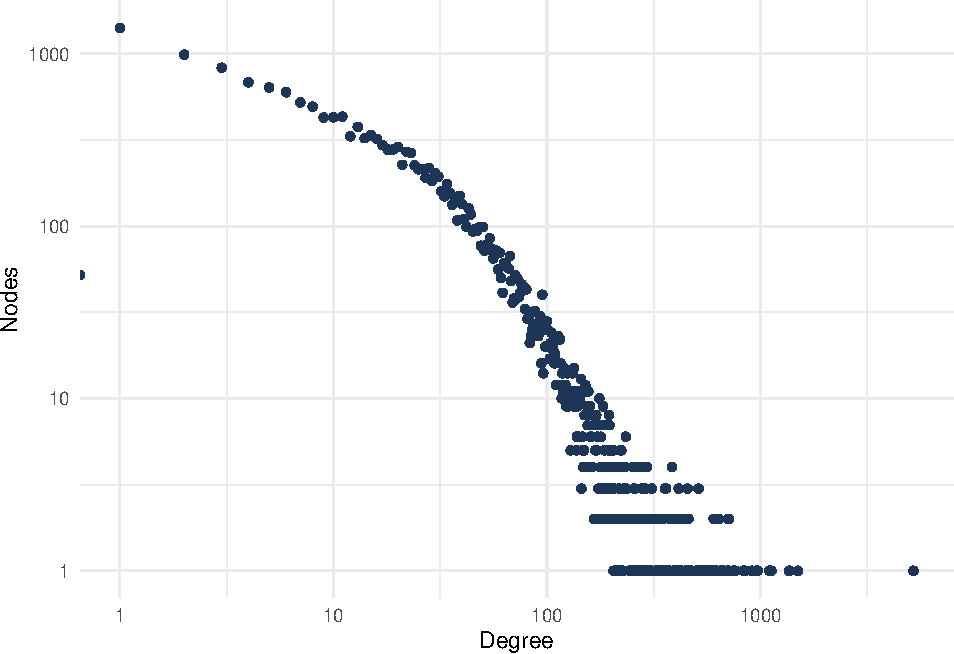
\includegraphics{NetMed_files/figure-latex/degree-distribution-1.pdf}
\caption{\label{fig:degree-distribution}PPI Degree Distribution}
\end{figure}

Most of the proteins have few connections, and very few proteins have lots of connections. Who's that protein?

\begin{Shaded}
\begin{Highlighting}[]
\FunctionTok{degree}\NormalTok{(gPPI) }\SpecialCharTok{\%\textgreater{}\%} 
  \FunctionTok{as.data.frame}\NormalTok{() }\SpecialCharTok{\%\textgreater{}\%} 
  \FunctionTok{arrange}\NormalTok{(}\FunctionTok{desc}\NormalTok{(.)) }\SpecialCharTok{\%\textgreater{}\%}
  \FunctionTok{filter}\NormalTok{(. }\SpecialCharTok{\textgreater{}} \DecValTok{1000}\NormalTok{) }\SpecialCharTok{\%\textgreater{}\%} 
\NormalTok{  knitr}\SpecialCharTok{::}\FunctionTok{kable}\NormalTok{()}
\end{Highlighting}
\end{Shaded}

\begin{tabular}{l|r}
\hline
  & .\\
\hline
UBC & 5199\\
\hline
ETS1 & 1496\\
\hline
GATA2 & 1369\\
\hline
CTCF & 1361\\
\hline
EP300 & 1124\\
\hline
MYC & 1107\\
\hline
AR & 1099\\
\hline
\end{tabular}

\hypertarget{exercises}{%
\subsection{Exercises}\label{exercises}}

Now is your turn. Spend some minutes understanding the data and getting some familiarity with it.

\begin{enumerate}
\def\labelenumi{\arabic{enumi}.}
\item
  What are the top 10 genes with higher degree?
\item
  Are those genes connected?
\end{enumerate}

\hypertarget{GDA}{%
\section{Gene Disease Association}\label{GDA}}

A Gene-Disease-Association (GDA) database are typically used to understand the association of genes to diseases, and model the underlying mechanisms of complex diseases. Those associations often come from GWAS studies and knock-out studies.

\hypertarget{commonly-used-data-sources-for-gdas}{%
\subsection{Commonly used data sources for GDAs}\label{commonly-used-data-sources-for-gdas}}

As PPIs, GDAs can be found from different sources and with different evidences for each Gene-Disease association. I list here some well known databases for that.

\begin{itemize}
\item
  CTD -- Curated scientific literature \citep{davis2020}
\item
  OMIM -- Curated scientific literature \citep{mckusick2007}
\item
  DisGeNet -- Based on OMIM, ClinVar and other data bases \citep{piñero2019}
\item
  Orphanet -- Validated - and non validated - GDAs
\item
  ClinGen -- Validated - and non validated - GDAs \citep{rehm2015}
\item
  ClinVar -- Different levels of evidence \citep{landrum2019}
\item
  GWAS catalogue -- GWAS associations to diseases \citep{buniello2018}
\item
  PheGenI -- GWAS associations to diseases \citep{ramos2013}
\item
  lncRNADisease -- Experimental validated lncRNAs in diseases \citep{chen2012}
\item
  HMDD -- Experimental validated miRNAs in diseases \citep{huang2018}
\end{itemize}

\hypertarget{understanding-a-gda-dataset}{%
\subsection{Understanding a GDA dataset}\label{understanding-a-gda-dataset}}

We will use in this workshop Gene-Disease-Association from DisGeNet. And can be \href{https://github.com/deisygysi/NetMed_Workshop/blob/master/data/curated_gene_disease_associations.tsv}{found here}.

Similar to the PPI, let us first get some familiarity with the data, before we are able to perform any analysis.

Let's read in the data and again, do some basic statistics.

\begin{Shaded}
\begin{Highlighting}[]
\NormalTok{GDA }\OtherTok{=} \FunctionTok{fread}\NormalTok{(}\AttributeTok{file =} \StringTok{\textquotesingle{}data/curated\_gene\_disease\_associations.tsv\textquotesingle{}}\NormalTok{, }\AttributeTok{sep =} \StringTok{\textquotesingle{}}\SpecialCharTok{\textbackslash{}t}\StringTok{\textquotesingle{}}\NormalTok{)}

\FunctionTok{head}\NormalTok{(GDA)}
\end{Highlighting}
\end{Shaded}

\begin{tabular}{r|l|r|r|l|l|l|l|l|r|r|r|r|r|r|l}
\hline
geneId & geneSymbol & DSI & DPI & diseaseId & diseaseName & diseaseType & diseaseClass & diseaseSemanticType & score & EI & YearInitial & YearFinal & NofPmids & NofSnps & source\\
\hline
1 & A1BG & 0.700 & 0.538 & C0019209 & Hepatomegaly & phenotype & C23;C06 & Finding & 0.30 & 1.000 & 2017 & 2017 & 1 & 0 & CTD\_human\\
\hline
1 & A1BG & 0.700 & 0.538 & C0036341 & Schizophrenia & disease & F03 & Mental or Behavioral Dysfunction & 0.30 & 1.000 & 2015 & 2015 & 1 & 0 & CTD\_human\\
\hline
2 & A2M & 0.529 & 0.769 & C0002395 & Alzheimer's Disease & disease & C10;F03 & Disease or Syndrome & 0.50 & 0.769 & 1998 & 2018 & 3 & 0 & CTD\_human\\
\hline
2 & A2M & 0.529 & 0.769 & C0007102 & Malignant tumor of colon & disease & C06;C04 & Neoplastic Process & 0.31 & 1.000 & 2004 & 2019 & 1 & 0 & CTD\_human\\
\hline
2 & A2M & 0.529 & 0.769 & C0009375 & Colonic Neoplasms & group & C06;C04 & Neoplastic Process & 0.30 & 1.000 & 2004 & 2004 & 1 & 0 & CTD\_human\\
\hline
2 & A2M & 0.529 & 0.769 & C0011265 & Presenile dementia & disease & C10;F03 & Mental or Behavioral Dysfunction & 0.30 & 1.000 & 1998 & 2004 & 3 & 0 & CTD\_human\\
\hline
\end{tabular}

The first thing to notice is the inconsistency with the disease names, in order to be able to work with it, let's first put every disease to lower-case.

\begin{Shaded}
\begin{Highlighting}[]
\NormalTok{Cleaned\_GDA }\OtherTok{=}\NormalTok{ GDA }\SpecialCharTok{\%\textgreater{}\%} \FunctionTok{filter}\NormalTok{(diseaseType }\SpecialCharTok{==} \StringTok{\textquotesingle{}disease\textquotesingle{}}\NormalTok{) }\SpecialCharTok{\%\textgreater{}\%}
  \FunctionTok{mutate}\NormalTok{(}\AttributeTok{diseaseName =} \FunctionTok{tolower}\NormalTok{(diseaseName)) }\SpecialCharTok{\%\textgreater{}\%}
  \FunctionTok{select}\NormalTok{(geneSymbol, diseaseName, diseaseSemanticType) }\SpecialCharTok{\%\textgreater{}\%}
  \FunctionTok{unique}\NormalTok{() }

\FunctionTok{dim}\NormalTok{(Cleaned\_GDA)}
\end{Highlighting}
\end{Shaded}

\begin{verbatim}
## [1] 60478     3
\end{verbatim}

\begin{Shaded}
\begin{Highlighting}[]
\FunctionTok{dim}\NormalTok{(GDA)}
\end{Highlighting}
\end{Shaded}

\begin{verbatim}
## [1] 84038    16
\end{verbatim}

\begin{Shaded}
\begin{Highlighting}[]
\NormalTok{numGenes }\OtherTok{=}\NormalTok{ Cleaned\_GDA }\SpecialCharTok{\%\textgreater{}\%} 
  \FunctionTok{group\_by}\NormalTok{(diseaseName) }\SpecialCharTok{\%\textgreater{}\%}
  \FunctionTok{summarise}\NormalTok{(}\AttributeTok{numGenes =} \FunctionTok{n}\NormalTok{()) }\SpecialCharTok{\%\textgreater{}\%}
  \FunctionTok{ungroup}\NormalTok{() }\SpecialCharTok{\%\textgreater{}\%}
  \FunctionTok{group\_by}\NormalTok{(numGenes) }\SpecialCharTok{\%\textgreater{}\%}
  \FunctionTok{summarise}\NormalTok{(}\AttributeTok{numDiseases =} \FunctionTok{n}\NormalTok{())}
\end{Highlighting}
\end{Shaded}

Let's also understand the degree distribution of the diseases.

\begin{Shaded}
\begin{Highlighting}[]
\FunctionTok{ggplot}\NormalTok{(numGenes) }\SpecialCharTok{+}
  \FunctionTok{aes}\NormalTok{(}\AttributeTok{x =}\NormalTok{ numGenes, }\AttributeTok{y =}\NormalTok{ numDiseases) }\SpecialCharTok{+}
  \FunctionTok{geom\_point}\NormalTok{(}\AttributeTok{colour =} \StringTok{"\#1d3557"}\NormalTok{) }\SpecialCharTok{+}
  \FunctionTok{scale\_x\_continuous}\NormalTok{(}\AttributeTok{trans =} \StringTok{"log10"}\NormalTok{) }\SpecialCharTok{+}
  \FunctionTok{scale\_y\_continuous}\NormalTok{(}\AttributeTok{trans =} \StringTok{"log10"}\NormalTok{) }\SpecialCharTok{+}
  \FunctionTok{labs}\NormalTok{(}\AttributeTok{x =} \StringTok{"Genes"}\NormalTok{, }\AttributeTok{y =} \StringTok{"Diseases"}\NormalTok{)}\SpecialCharTok{+}
  \FunctionTok{theme\_minimal}\NormalTok{()}
\end{Highlighting}
\end{Shaded}

\begin{figure}
\centering
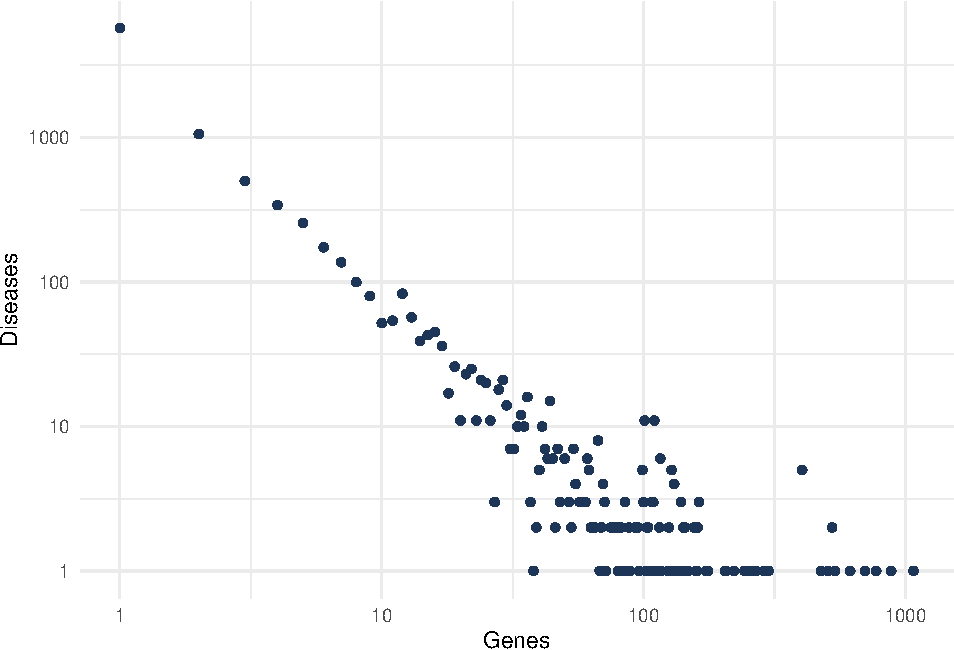
\includegraphics{NetMed_files/figure-latex/unnamed-chunk-11-1.pdf}
\caption{\label{fig:unnamed-chunk-11}Gene-Disease degree distribution}
\end{figure}

Because we want to focus in well studied diseases, and also that are known to be complex diseases, let's filter for diseases with at least 10 genes.

\begin{Shaded}
\begin{Highlighting}[]
\NormalTok{Cleaned\_GDA }\SpecialCharTok{\%\textless{}\textgreater{}\%} 
  \FunctionTok{group\_by}\NormalTok{(diseaseName) }\SpecialCharTok{\%\textgreater{}\%}
  \FunctionTok{mutate}\NormalTok{(}\AttributeTok{numGenes =} \FunctionTok{n}\NormalTok{()) }\SpecialCharTok{\%\textgreater{}\%}
  \FunctionTok{filter}\NormalTok{(numGenes }\SpecialCharTok{\textgreater{}} \DecValTok{10}\NormalTok{)}

\NormalTok{Cleaned\_GDA}\SpecialCharTok{$}\NormalTok{diseaseName }\SpecialCharTok{\%\textgreater{}\%} \FunctionTok{unique}\NormalTok{() }\SpecialCharTok{\%\textgreater{}\%}  \FunctionTok{length}\NormalTok{()}
\end{Highlighting}
\end{Shaded}

\begin{verbatim}
## [1] 920
\end{verbatim}

\hypertarget{exercises-1}{%
\subsection{Exercises}\label{exercises-1}}

Now is your turn. Spend some minutes understanding the data and getting some familiarity with it.

\begin{enumerate}
\def\labelenumi{\arabic{enumi}.}
\item
  What are the top 10 genes mostly involved with diseases? What are those diseases?
\item
  What are the top 10 highly polygenic diseases?
\item
  What are the top 10 highly polygenic disease classes?
\end{enumerate}

\hypertarget{DTs}{%
\section{Drug-Targets}\label{DTs}}

A \emph{druggable} target is a protein, peptide or nucleic acid that has activity which can be modulated by a drug. A \emph{drug} can be any small molecular weight chemical compound (SMOL) or a biologic (BIOL), such as an antibody or a recombinant protein that can treat a disease or a sympthom.

\hypertarget{properties-of-an-ideal-drug-target}{%
\subsection{Properties of an ideal drug target:}\label{properties-of-an-ideal-drug-target}}

A drug-target has a couple of proprieties that are highly desired when constructing the drug \citep{Gashaw2011}:

\begin{itemize}
\item
  Target is disease-modifying and/or has a proven function in the pathophysiology of a disease.
\item
  Modulation of the target is less important under physiological conditions or in other diseases.
\item
  If the druggability is not obvious (e.g.~as for kinases) a 3D-structure for the target protein or a close homolog should be available for a druggability assessment.
\item
  Target has a favorable `assayability' enabling high throughput screening.
\item
  Target expression is not uniformly distributed throughout the body.
\item
  A target/disease-specific biomarker exists to monitor therapeutic efficacy.
\item
  Favorable prediction of potential side effects according to phenotype data (e.g.~in k.o. mice or genetic mutation databases).
\item
  Target has a favorable IP situation (no competitors on target, freedom to operate).
\end{itemize}

\hypertarget{commonly-used-data-sources-for-gdas-1}{%
\subsection{Commonly used data sources for GDAs}\label{commonly-used-data-sources-for-gdas-1}}

There are a couple of really good data sets that report drug-target interactions, I list here three good examples:

\begin{enumerate}
\def\labelenumi{\arabic{enumi}.}
\item
  DrugBank \citep{Wishart2006, wishart2017}
\item
  CTD \citep{davis2020}
\item
  Broad Institute Drug Repositioning Hub \citep{corsello2017}
\end{enumerate}

\hypertarget{understanding-a-drug-target-dataset}{%
\subsection{Understanding a Drug-Target dataset}\label{understanding-a-drug-target-dataset}}

For this workshop we will use the drug bank drug-target dataset, and can be \href{https://github.com/deisygysi/NetMed_Workshop/blob/master/data/DB_DrugTargets_1201.csv}{found here}. This dataset is from Drug-Bank, and has been previously parsed for your convenience. The original file is an XML file, and needs to be carefully handled to get information needed.

Similar to the PPI and the GDA, let us understand a little bit of the data set, and what kind of information we have here.

\begin{Shaded}
\begin{Highlighting}[]
\NormalTok{DT }\OtherTok{=} \FunctionTok{fread}\NormalTok{(}\AttributeTok{file =} \StringTok{\textquotesingle{}data/DB\_DrugTargets\_1201.csv\textquotesingle{}}\NormalTok{)}

\FunctionTok{head}\NormalTok{(DT)}
\end{Highlighting}
\end{Shaded}

\begin{tabular}{l|l|l|l|l|l|l|l|l|l|l|l|l|l}
\hline
i & ID & Name & Started\_commer & Ended\_commer & ATC & State & Approved & Gene\_Target & DB\_id & name & organism & Type & known\_action\\
\hline
1 & DB00001 & Lepirudin & 1997-03-13 & 2012-07-27 & B01AE & liquid & approved & F2 & BE0000048 & Prothrombin & Humans & Polypeptide & yes\\
\hline
2 & DB00002 & Cetuximab & 2004-06-29 & NA & L01XC & liquid & approved & EGFR & BE0002098 & Low affinity immunoglobulin gamma Fc region receptor II-a & Humans & Polypeptide & unknown\\
\hline
2 & DB00002 & Cetuximab & 2004-06-29 & NA & L01XC & liquid & approved & FCGR3B & BE0002098 & Low affinity immunoglobulin gamma Fc region receptor II-a & Humans & Polypeptide & unknown\\
\hline
2 & DB00002 & Cetuximab & 2004-06-29 & NA & L01XC & liquid & approved & C1QA & BE0002098 & Low affinity immunoglobulin gamma Fc region receptor II-a & Humans & Polypeptide & unknown\\
\hline
2 & DB00002 & Cetuximab & 2004-06-29 & NA & L01XC & liquid & approved & C1QB & BE0002098 & Low affinity immunoglobulin gamma Fc region receptor II-a & Humans & Polypeptide & unknown\\
\hline
2 & DB00002 & Cetuximab & 2004-06-29 & NA & L01XC & liquid & approved & C1QC & BE0002098 & Low affinity immunoglobulin gamma Fc region receptor II-a & Humans & Polypeptide & unknown\\
\hline
\end{tabular}

\begin{Shaded}
\begin{Highlighting}[]
\NormalTok{Cleaned\_DT }\OtherTok{=}\NormalTok{ DT }\SpecialCharTok{\%\textgreater{}\%} 
  \FunctionTok{filter}\NormalTok{(organism }\SpecialCharTok{==} \StringTok{\textquotesingle{}Humans\textquotesingle{}}\NormalTok{) }\SpecialCharTok{\%\textgreater{}\%}
  \FunctionTok{select}\NormalTok{(Gene\_Target, Name,ID, Type, known\_action) }\SpecialCharTok{\%\textgreater{}\%}
  \FunctionTok{unique}\NormalTok{() }

\FunctionTok{dim}\NormalTok{(Cleaned\_DT)}
\end{Highlighting}
\end{Shaded}

\begin{verbatim}
## [1] 22931     5
\end{verbatim}

\begin{Shaded}
\begin{Highlighting}[]
\FunctionTok{dim}\NormalTok{(DT)}
\end{Highlighting}
\end{Shaded}

\begin{verbatim}
## [1] 26817    16
\end{verbatim}

\begin{Shaded}
\begin{Highlighting}[]
\FunctionTok{head}\NormalTok{(Cleaned\_DT)}
\end{Highlighting}
\end{Shaded}

\begin{verbatim}
##    Gene_Target      Name      ID        Type known_action
## 1:          F2 Lepirudin DB00001 Polypeptide          yes
## 2:        EGFR Cetuximab DB00002 Polypeptide      unknown
## 3:      FCGR3B Cetuximab DB00002 Polypeptide      unknown
## 4:        C1QA Cetuximab DB00002 Polypeptide      unknown
## 5:        C1QB Cetuximab DB00002 Polypeptide      unknown
## 6:        C1QC Cetuximab DB00002 Polypeptide      unknown
\end{verbatim}

\begin{Shaded}
\begin{Highlighting}[]
\NormalTok{TargetDist }\OtherTok{=}\NormalTok{ Cleaned\_DT }\SpecialCharTok{\%\textgreater{}\%} 
  \FunctionTok{group\_by}\NormalTok{(Gene\_Target) }\SpecialCharTok{\%\textgreater{}\%}
  \FunctionTok{summarise}\NormalTok{(}\AttributeTok{numDrugs =} \FunctionTok{n}\NormalTok{()) }

\NormalTok{DrugDist }\OtherTok{=}\NormalTok{ Cleaned\_DT }\SpecialCharTok{\%\textgreater{}\%} 
  \FunctionTok{group\_by}\NormalTok{(ID) }\SpecialCharTok{\%\textgreater{}\%}
  \FunctionTok{summarise}\NormalTok{(}\AttributeTok{numTargets =} \FunctionTok{n}\NormalTok{()) }
\end{Highlighting}
\end{Shaded}

\begin{Shaded}
\begin{Highlighting}[]
\FunctionTok{ggplot}\NormalTok{(TargetDist) }\SpecialCharTok{+}
  \FunctionTok{aes}\NormalTok{(}\AttributeTok{x =}\NormalTok{ numDrugs) }\SpecialCharTok{+}
  \FunctionTok{geom\_histogram}\NormalTok{(}\AttributeTok{colour =} \StringTok{"\#1d3557"}\NormalTok{, }\AttributeTok{fill =} \StringTok{"\#a8dadc"}\NormalTok{ ) }\SpecialCharTok{+}
  \FunctionTok{labs}\NormalTok{(}\AttributeTok{x =} \StringTok{"Targets"}\NormalTok{, }\AttributeTok{y =} \StringTok{"Drugs"}\NormalTok{)}\SpecialCharTok{+}
  \FunctionTok{theme\_minimal}\NormalTok{()}
\end{Highlighting}
\end{Shaded}

\begin{figure}
\centering
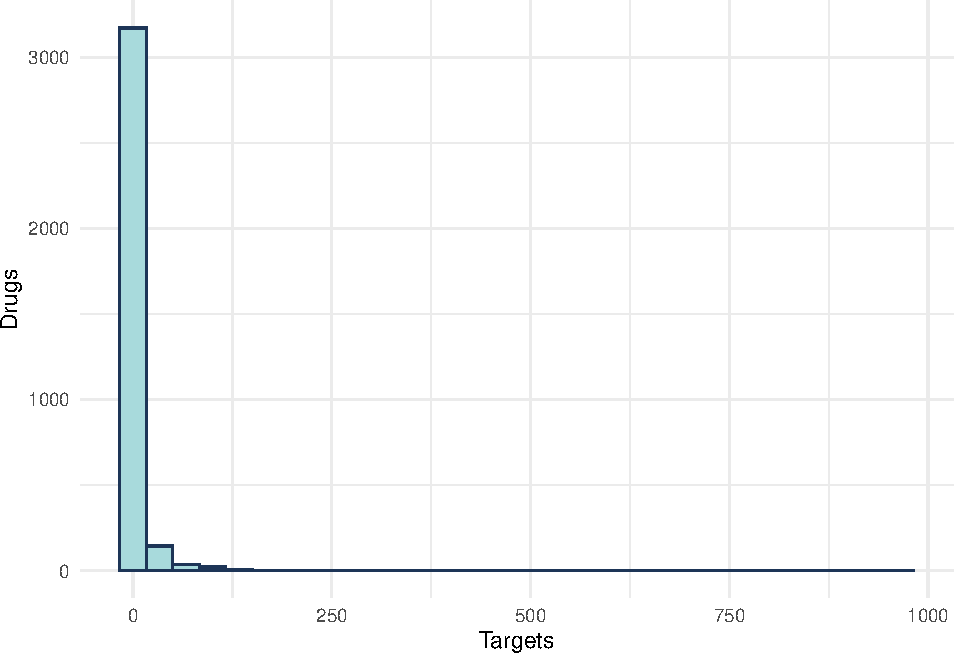
\includegraphics{NetMed_files/figure-latex/unnamed-chunk-17-1.pdf}
\caption{\label{fig:unnamed-chunk-17}Target distribution}
\end{figure}

Which Target is the most targetted gene?

\begin{Shaded}
\begin{Highlighting}[]
\NormalTok{TargetDist }\SpecialCharTok{\%\textgreater{}\%}
  \FunctionTok{arrange}\NormalTok{(}\FunctionTok{desc}\NormalTok{(numDrugs)) }\SpecialCharTok{\%\textgreater{}\%}
  \FunctionTok{filter}\NormalTok{(numDrugs }\SpecialCharTok{\textgreater{}} \DecValTok{400}\NormalTok{)}
\end{Highlighting}
\end{Shaded}

\begin{verbatim}
## # A tibble: 2 x 2
##   Gene_Target numDrugs
##   <chr>          <int>
## 1 CYP3A4           966
## 2 ABCB1            524
\end{verbatim}

\begin{Shaded}
\begin{Highlighting}[]
\FunctionTok{ggplot}\NormalTok{(DrugDist) }\SpecialCharTok{+}
  \FunctionTok{aes}\NormalTok{(}\AttributeTok{x =}\NormalTok{ numTargets) }\SpecialCharTok{+}
  \FunctionTok{geom\_histogram}\NormalTok{(}\AttributeTok{colour =} \StringTok{"\#1d3557"}\NormalTok{, }\AttributeTok{fill =} \StringTok{"\#a8dadc"}\NormalTok{ ) }\SpecialCharTok{+}
  \FunctionTok{labs}\NormalTok{(}\AttributeTok{y =} \StringTok{"Targets"}\NormalTok{, }\AttributeTok{x =} \StringTok{"Drugs"}\NormalTok{)}\SpecialCharTok{+}
  \FunctionTok{theme\_minimal}\NormalTok{()}
\end{Highlighting}
\end{Shaded}

\begin{figure}
\centering
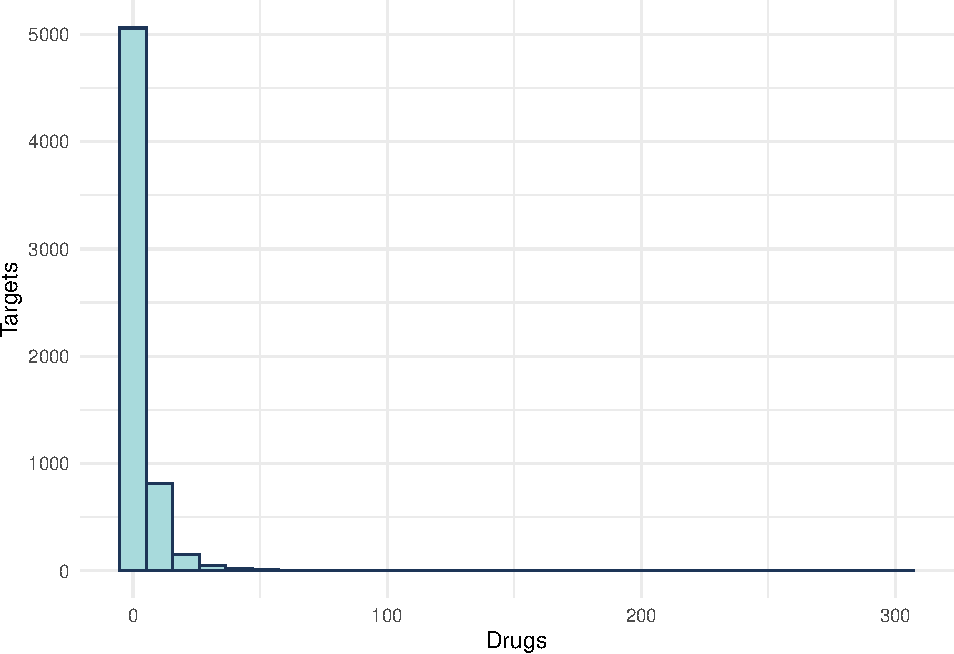
\includegraphics{NetMed_files/figure-latex/unnamed-chunk-19-1.pdf}
\caption{\label{fig:unnamed-chunk-19}Drug distribution}
\end{figure}

\hypertarget{exercises-2}{%
\subsection{Exercises}\label{exercises-2}}

Let us understand a little bit more about the data.

\begin{enumerate}
\def\labelenumi{\arabic{enumi}.}
\item
  What are the top 10 genes mostly targeted by drugs? Are they types are they mostly?
\item
  What are the top 10 most promiscuous drugs? What are their indication?
\end{enumerate}

\hypertarget{methods}{%
\chapter{Methods fo Disease Module Identification and Disease Similarity}\label{methods}}

In this chapter, I will introduce the main methods used in Network Medicine. We will start by understanding what a Disease Module is (Session \ref{diseasemodule}), how can we calculate its significance and also understand its importance. We next will explore the disease separation (Session \ref{dissep}), how to calculate, make interpretations.

\hypertarget{diseasemodule}{%
\section{Disease Module}\label{diseasemodule}}

In biological networks often genes involved in the same topological communities are also associated with similar biological processes \citep{Ahn2010}. It also reflects on \emph{how diseases localized themselves in the interaction}; meaning that disease modules are highly localized in specific network neighborhoods \citep{Menche2015} (Figure \ref{fig:diseasemodule}).

\hypertarget{largest-connected-component}{%
\subsection{Largest connected component}\label{largest-connected-component}}

The size of the largest connected component (LCC) is the number of nodes that form a connected subgraph (in our case, it is the number of proteins that are interconnected in the PPI). Many properties of this quantity allow us to understand how a particular disease interacts with the interactome. It is important to note here that this measure is highly dependent on the completeness of an interactome. If a link between a protein and their counterparts is unknown -- therefore missing -- we might say that that particular node is not involved in a disease module (or that the LCC is not significant).

\begin{figure}
\centering
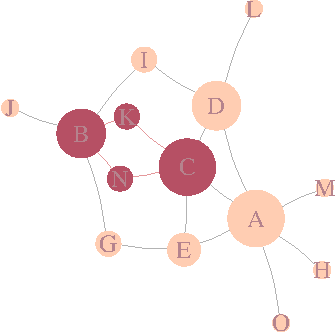
\includegraphics{NetMed_files/figure-latex/diseasemodule-1.pdf}
\caption{\label{fig:diseasemodule}Disease-Module. A schematic of a PPI, in pink we see genes associated with a disease, forming a connected component of size 4.}
\end{figure}

However, just computing this number might not be informative, and it is expected a randomness. To calculate this randomness, we often calculate the significance of the LCC by selecting proteins in the interactome with similar degrees (aka degree preserving randomization).

To calculate the significance of the LCC one can calculate its Z-Score or simply calculate the empirical probability under the curve from the empirical distribution. The Z-score is given by:

\[
Z-Score_{LCC} = \frac{LCC - \mu_{LCC}}{\sigma_{LCC}}
\]

\hypertarget{example-in-real-data}{%
\subsection{Example in real data}\label{example-in-real-data}}

Our first task now, is to understand if some diseases, from our \texttt{Cleaned\_GDA} are able to form a Disease-Module. Let's start doing it for Schizophrenia and later we will add some more diseases.

The idea now is: Gather the genes associated to our disease in the data, find them in the PPI, check if they form a connected component, check the significance of the component and visualize the Disease-Module.

\begin{Shaded}
\begin{Highlighting}[]
\CommentTok{\# First, let\textquotesingle{}s attach all packages we will need.}
\FunctionTok{require}\NormalTok{(NetSci)}
\FunctionTok{require}\NormalTok{(magrittr)}
\FunctionTok{require}\NormalTok{(dplyr)}
\FunctionTok{require}\NormalTok{(igraph)}
\end{Highlighting}
\end{Shaded}

\begin{Shaded}
\begin{Highlighting}[]
\CommentTok{\#First, let\textquotesingle{}s select genes that are associated with Schizophrenia.}

\NormalTok{SCZ\_Genes }\OtherTok{=} 
\NormalTok{  Cleaned\_GDA }\SpecialCharTok{\%\textgreater{}\%} 
  \FunctionTok{filter}\NormalTok{(diseaseName }\SpecialCharTok{\%in\%} \StringTok{\textquotesingle{}schizophrenia\textquotesingle{}}\NormalTok{) }\SpecialCharTok{\%\textgreater{}\%}
  \FunctionTok{pull}\NormalTok{(geneSymbol) }\SpecialCharTok{\%\textgreater{}\%} 
  \FunctionTok{unique}\NormalTok{()}

\CommentTok{\# Next, let\textquotesingle{}s see how they are localized in the PPI.}
\CommentTok{\# Fist, we have to make sure all genes are in the PPI.}
\CommentTok{\# Later, we calculate the LCC.}
\CommentTok{\# And lastly, let\textquotesingle{}s visualize it.}

\NormalTok{SCZ\_PPI }\OtherTok{=}\NormalTok{ SCZ\_Genes[SCZ\_Genes }\SpecialCharTok{\%in\%} \FunctionTok{V}\NormalTok{(gPPI)}\SpecialCharTok{$}\NormalTok{name]}
\NormalTok{gScz }\OtherTok{=}\NormalTok{ gPPI }\SpecialCharTok{\%\textgreater{}\%} \FunctionTok{induced.subgraph}\NormalTok{(., SCZ\_PPI)}

\FunctionTok{components}\NormalTok{(gScz)}
\end{Highlighting}
\end{Shaded}

\begin{Shaded}
\begin{Highlighting}[]
\FunctionTok{components}\NormalTok{(gScz)}\SpecialCharTok{$}\NormalTok{csize }\SpecialCharTok{\%\textgreater{}\%}\NormalTok{ max}
\end{Highlighting}
\end{Shaded}

\begin{verbatim}
## [1] 683
\end{verbatim}

\begin{Shaded}
\begin{Highlighting}[]
\CommentTok{\# The size of the LCC is 683. But... How does it compare to a random selection genes?}

\NormalTok{LCC\_scz }\OtherTok{=} \FunctionTok{LCC\_Significance}\NormalTok{(}\AttributeTok{N =} \DecValTok{10}\NormalTok{, }\AttributeTok{Targets =}\NormalTok{ SCZ\_PPI,}
                           \AttributeTok{G =}\NormalTok{ gPPI)}
\FunctionTok{Histogram\_LCC}\NormalTok{(LCC\_scz)}
\end{Highlighting}
\end{Shaded}

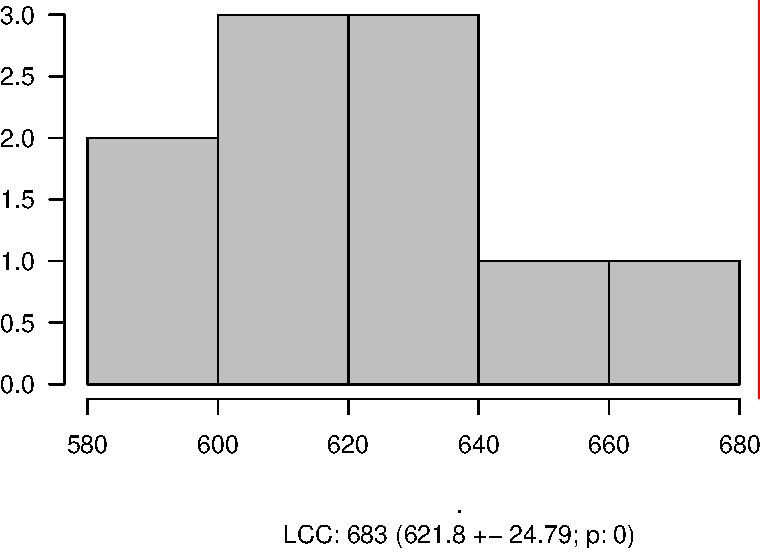
\includegraphics{NetMed_files/figure-latex/unnamed-chunk-23-1.pdf}

\begin{Shaded}
\begin{Highlighting}[]
\NormalTok{gScz }
\end{Highlighting}
\end{Shaded}

\begin{verbatim}
## IGRAPH 47034ad UN-- 846 2564 -- 
## + attr: name (v/c)
## + edges from 47034ad (vertex names):
##  [1] PI4KA  --SP1    F2     --SP1    DNM1   --CTCF   GSK3B  --HSPA1A
##  [5] DNM1   --GRB2   SP1    --GRB2   MET    --GRB2   GSK3B  --MAPK14
##  [9] SP1    --MAPK14 CTCF   --MAPK14 GRB2   --MAPK14 MET    --ACTB  
## [13] GRB2   --ACTB   MAPK14 --ACTB   GSK3B  --SOX10  SP1    --SOX10 
## [17] PAX6   --SOX10  SP1    --CCNA2  ACTB   --MTNR1A ACTB   --GSN   
## [21] PI4KA  --JUN    GSK3B  --JUN    SMARCA2--JUN    SP1    --JUN   
## [25] MAPK14 --JUN    SOX10  --JUN    GSK3B  --ESR1   SMARCA2--ESR1  
## [29] SP1    --ESR1   HSPA1A --ESR1   FMR1   --ESR1   MAPK14 --ESR1  
## + ... omitted several edges
\end{verbatim}

\begin{Shaded}
\begin{Highlighting}[]
\FunctionTok{V}\NormalTok{(gScz)}\SpecialCharTok{$}\NormalTok{size }\OtherTok{=} \FunctionTok{degree}\NormalTok{(gScz) }\SpecialCharTok{\%\textgreater{}\%} 
\NormalTok{  CoDiNA}\SpecialCharTok{::}\FunctionTok{normalize}\NormalTok{()}
\FunctionTok{V}\NormalTok{(gScz)}\SpecialCharTok{$}\NormalTok{size }\OtherTok{=}\NormalTok{ (}\FunctionTok{V}\NormalTok{(gScz)}\SpecialCharTok{$}\NormalTok{size }\SpecialCharTok{+} \FloatTok{0.1}\NormalTok{)}\SpecialCharTok{*}\DecValTok{5}
\FunctionTok{V}\NormalTok{(gScz)}\SpecialCharTok{$}\NormalTok{color }\OtherTok{=} \StringTok{\textquotesingle{}\#83c5be\textquotesingle{}}
\FunctionTok{V}\NormalTok{(gScz)}\SpecialCharTok{$}\NormalTok{frame.color }\OtherTok{=} \StringTok{\textquotesingle{}\#006d77\textquotesingle{}}
\FunctionTok{V}\NormalTok{(gScz)}\SpecialCharTok{$}\NormalTok{label }\OtherTok{=} \FunctionTok{ifelse}\NormalTok{(}\FunctionTok{V}\NormalTok{(gScz)}\SpecialCharTok{$}\NormalTok{size  }\SpecialCharTok{\textgreater{}} \DecValTok{4}\NormalTok{, }\FunctionTok{V}\NormalTok{(gScz)}\SpecialCharTok{$}\NormalTok{name, }\ConstantTok{NA}\NormalTok{ )}
\FunctionTok{V}\NormalTok{(gScz)}\SpecialCharTok{$}\NormalTok{label.color }\OtherTok{=} \StringTok{\textquotesingle{}\#e29578\textquotesingle{}}

\FunctionTok{E}\NormalTok{(gScz)}\SpecialCharTok{$}\NormalTok{width }\OtherTok{=} \FunctionTok{edge.betweenness}\NormalTok{(gScz, }\AttributeTok{directed =}\NormalTok{ F) }\SpecialCharTok{\%\textgreater{}\%}\NormalTok{ CoDiNA}\SpecialCharTok{::}\FunctionTok{normalize}\NormalTok{()}
\FunctionTok{E}\NormalTok{(gScz)}\SpecialCharTok{$}\NormalTok{width }\OtherTok{=} \FunctionTok{E}\NormalTok{(gScz)}\SpecialCharTok{$}\NormalTok{width }\SpecialCharTok{+} \FloatTok{0.01}
\FunctionTok{E}\NormalTok{(gScz)}\SpecialCharTok{$}\NormalTok{weight }\OtherTok{=} \FunctionTok{E}\NormalTok{(gScz)}\SpecialCharTok{$}\NormalTok{width}
\FunctionTok{plot}\NormalTok{(gScz)}
\end{Highlighting}
\end{Shaded}

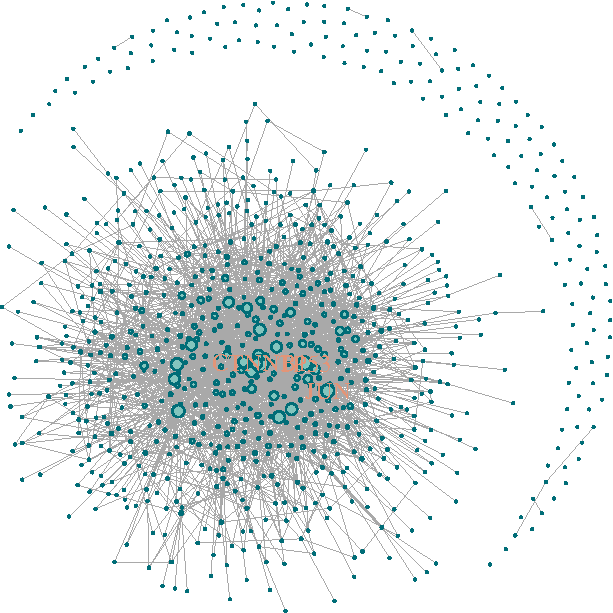
\includegraphics{NetMed_files/figure-latex/unnamed-chunk-24-1.pdf}

\begin{Shaded}
\begin{Highlighting}[]
\NormalTok{gScz }\SpecialCharTok{\%\textless{}\textgreater{}\%} \FunctionTok{delete.vertices}\NormalTok{(., }\FunctionTok{degree}\NormalTok{(.) }\SpecialCharTok{==} \DecValTok{0}\NormalTok{)}

\FunctionTok{V}\NormalTok{(gScz)}\SpecialCharTok{$}\NormalTok{size }\OtherTok{=} \FunctionTok{degree}\NormalTok{(gScz) }\SpecialCharTok{\%\textgreater{}\%} 
\NormalTok{  CoDiNA}\SpecialCharTok{::}\FunctionTok{normalize}\NormalTok{()}
\FunctionTok{V}\NormalTok{(gScz)}\SpecialCharTok{$}\NormalTok{size }\OtherTok{=}\NormalTok{ (}\FunctionTok{V}\NormalTok{(gScz)}\SpecialCharTok{$}\NormalTok{size }\SpecialCharTok{+} \FloatTok{0.1}\NormalTok{)}\SpecialCharTok{*}\DecValTok{5}
\FunctionTok{V}\NormalTok{(gScz)}\SpecialCharTok{$}\NormalTok{color }\OtherTok{=} \StringTok{\textquotesingle{}\#83c5be\textquotesingle{}}
\FunctionTok{V}\NormalTok{(gScz)}\SpecialCharTok{$}\NormalTok{frame.color }\OtherTok{=} \StringTok{\textquotesingle{}\#006d77\textquotesingle{}}
\FunctionTok{V}\NormalTok{(gScz)}\SpecialCharTok{$}\NormalTok{label }\OtherTok{=} \FunctionTok{ifelse}\NormalTok{(}\FunctionTok{V}\NormalTok{(gScz)}\SpecialCharTok{$}\NormalTok{size  }\SpecialCharTok{\textgreater{}} \DecValTok{4}\NormalTok{, }\FunctionTok{V}\NormalTok{(gScz)}\SpecialCharTok{$}\NormalTok{name, }\ConstantTok{NA}\NormalTok{ )}
\FunctionTok{V}\NormalTok{(gScz)}\SpecialCharTok{$}\NormalTok{label.color }\OtherTok{=} \StringTok{\textquotesingle{}\#e29578\textquotesingle{}}

\FunctionTok{E}\NormalTok{(gScz)}\SpecialCharTok{$}\NormalTok{width }\OtherTok{=} \FunctionTok{edge.betweenness}\NormalTok{(gScz, }\AttributeTok{directed =}\NormalTok{ F) }\SpecialCharTok{\%\textgreater{}\%}\NormalTok{ CoDiNA}\SpecialCharTok{::}\FunctionTok{normalize}\NormalTok{()}
\FunctionTok{E}\NormalTok{(gScz)}\SpecialCharTok{$}\NormalTok{width }\OtherTok{=} \FunctionTok{E}\NormalTok{(gScz)}\SpecialCharTok{$}\NormalTok{width }\SpecialCharTok{+} \FloatTok{0.01}
\FunctionTok{E}\NormalTok{(gScz)}\SpecialCharTok{$}\NormalTok{weight }\OtherTok{=} \FunctionTok{E}\NormalTok{(gScz)}\SpecialCharTok{$}\NormalTok{width}
\FunctionTok{plot}\NormalTok{(gScz)}
\end{Highlighting}
\end{Shaded}

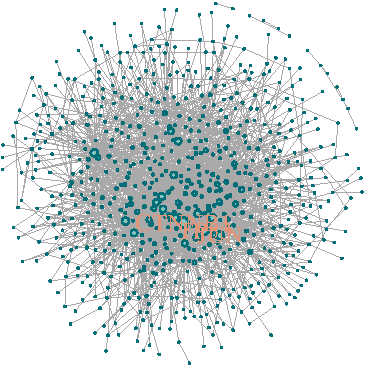
\includegraphics{NetMed_files/figure-latex/unnamed-chunk-25-1.pdf}

\hypertarget{exercises-3}{%
\subsection{Exercises}\label{exercises-3}}

\begin{enumerate}
\def\labelenumi{\arabic{enumi}.}
\item
  Calculate the LCC, and visualize the modules for the following diseases:

  \begin{itemize}
  \tightlist
  \item
    Autistic Disorder;
  \item
    Obesity;
  \item
    Hyperlipidemia;
  \item
    Rheumatoid Arthritis.
  \end{itemize}
\item
  Now choose any disease you are interested in and do the same thing.
\end{enumerate}

\hypertarget{gene-overlap}{%
\section{Gene Overlap}\label{gene-overlap}}

A first intuitive way to measure the overlap of two gene sets is by calculating its overlap, or its normalized overlap, the \textbf{Jaccard Index}. The Jaccard index is calculated by taking the ratio of \textbf{Intersection of two sets over Union of those sets}. The Jaccard coefficient measures similarity between finite sample sets, and is defined as the size of the intersection divided by the size of the union of the sample sets:

\[
J(A,B) = \frac{|A \cap B|}{|A \cup B|} = \frac{|A \cap B|}{|A| + |B| - |A \cap B|}
\]

Note that by design, \(0 \leq J(A,B) \leq 1\). If A and B are both empty, define \(J(A,B) = 1\)

Let's calculate the Jaccard Index for the 5 diseases we calculated its LCCs.

\begin{Shaded}
\begin{Highlighting}[]
\NormalTok{Dis\_Ex1 }\OtherTok{=} \FunctionTok{c}\NormalTok{(}\StringTok{\textquotesingle{}schizophrenia\textquotesingle{}}\NormalTok{,}
            \StringTok{"autistic disorder"}\NormalTok{, }
            \StringTok{\textquotesingle{}obesity\textquotesingle{}}\NormalTok{,}
            \StringTok{\textquotesingle{}hyperlipidemia\textquotesingle{}}\NormalTok{,}
            \StringTok{\textquotesingle{}rheumatoid arthritis\textquotesingle{}}\NormalTok{)}
\NormalTok{GDA\_Interest }\OtherTok{=}\NormalTok{ Cleaned\_GDA }\SpecialCharTok{\%\textgreater{}\%} 
  \FunctionTok{filter}\NormalTok{(diseaseName }\SpecialCharTok{\%in\%}\NormalTok{ Dis\_Ex1) }\SpecialCharTok{\%\textgreater{}\%}
  \FunctionTok{select}\NormalTok{(diseaseName, geneSymbol) }\SpecialCharTok{\%\textgreater{}\%}
  \FunctionTok{unique}\NormalTok{()}

\NormalTok{Jaccard\_Ex2 }\OtherTok{=} \FunctionTok{Jaccard}\NormalTok{(GDA\_Interest)}
\end{Highlighting}
\end{Shaded}

\begin{verbatim}
##   |                                                                              |                                                                      |   0%  |                                                                              |==============                                                        |  20%  |                                                                              |============================                                          |  40%  |                                                                              |==========================================                            |  60%  |                                                                              |========================================================              |  80%  |                                                                              |======================================================================| 100%
\end{verbatim}

\begin{Shaded}
\begin{Highlighting}[]
\NormalTok{Jaccard\_Ex2}
\end{Highlighting}
\end{Shaded}

\begin{verbatim}
##                   Node.1               Node.2 Jaccard.Index
##  1:        schizophrenia    autistic disorder   0.095785441
##  2:        schizophrenia              obesity   0.039159503
##  3:    autistic disorder              obesity   0.033259424
##  4:        schizophrenia rheumatoid arthritis   0.027210884
##  5:    autistic disorder rheumatoid arthritis   0.035714286
##  6:              obesity rheumatoid arthritis   0.029891304
##  7:        schizophrenia       hyperlipidemia   0.005586592
##  8:    autistic disorder       hyperlipidemia   0.007246377
##  9:              obesity       hyperlipidemia   0.052132701
## 10: rheumatoid arthritis       hyperlipidemia   0.000000000
\end{verbatim}

\begin{Shaded}
\begin{Highlighting}[]
\CommentTok{\# Let\textquotesingle{}s visualize the Venn diagram (Euler Diagram) of those overlaps. }

\FunctionTok{require}\NormalTok{(eulerr)}
\end{Highlighting}
\end{Shaded}

\begin{verbatim}
## Loading required package: eulerr
\end{verbatim}

\begin{Shaded}
\begin{Highlighting}[]
\NormalTok{Euler\_List }\OtherTok{=} \FunctionTok{list}\NormalTok{ (}
  \AttributeTok{SCZ =}\NormalTok{ GDA\_Interest}\SpecialCharTok{$}\NormalTok{geneSymbol[GDA\_Interest}\SpecialCharTok{$}\NormalTok{diseaseName }\SpecialCharTok{==} \StringTok{\textquotesingle{}schizophrenia\textquotesingle{}}\NormalTok{],}
                   
  \AttributeTok{ASD =}\NormalTok{ GDA\_Interest}\SpecialCharTok{$}\NormalTok{geneSymbol[GDA\_Interest}\SpecialCharTok{$}\NormalTok{diseaseName }\SpecialCharTok{==} \StringTok{\textquotesingle{}autistic disorder\textquotesingle{}}\NormalTok{],}
                   
  \AttributeTok{OB =}\NormalTok{ GDA\_Interest}\SpecialCharTok{$}\NormalTok{geneSymbol[GDA\_Interest}\SpecialCharTok{$}\NormalTok{diseaseName }\SpecialCharTok{==} \StringTok{\textquotesingle{}obesity\textquotesingle{}}\NormalTok{],}
                   
  \AttributeTok{HD =}\NormalTok{ GDA\_Interest}\SpecialCharTok{$}\NormalTok{geneSymbol[GDA\_Interest}\SpecialCharTok{$}\NormalTok{diseaseName }\SpecialCharTok{==} \StringTok{\textquotesingle{}hyperlipidemia\textquotesingle{}}\NormalTok{],}
                   
  \AttributeTok{RA =}\NormalTok{ GDA\_Interest}\SpecialCharTok{$}\NormalTok{geneSymbol[GDA\_Interest}\SpecialCharTok{$}\NormalTok{diseaseName }\SpecialCharTok{==} \StringTok{\textquotesingle{}rheumatoid arthritis\textquotesingle{}}\NormalTok{])}

\NormalTok{EULER }\OtherTok{=} \FunctionTok{euler}\NormalTok{(Euler\_List)}
\FunctionTok{plot}\NormalTok{(EULER, }\AttributeTok{quantities =} \ConstantTok{TRUE}\NormalTok{)}
\end{Highlighting}
\end{Shaded}

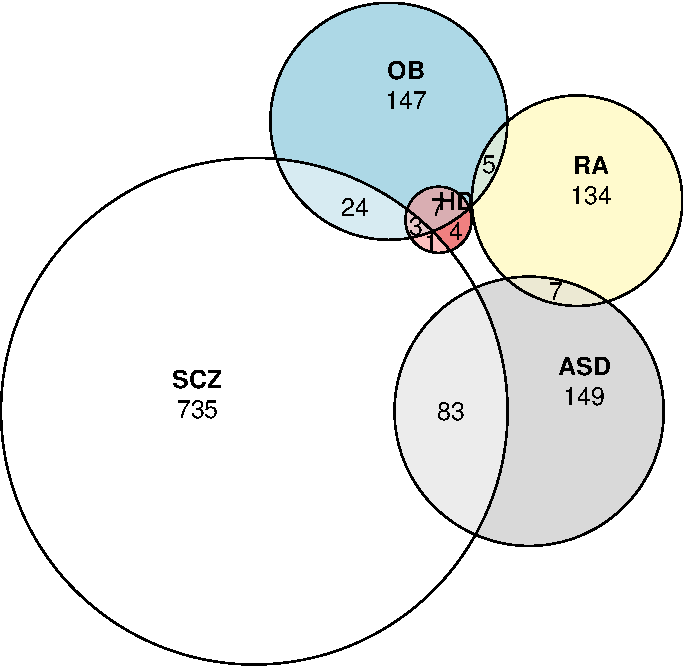
\includegraphics{NetMed_files/figure-latex/unnamed-chunk-27-1.pdf}

\hypertarget{dissep}{%
\section{Disease Separation}\label{dissep}}

When looking into the Jaccard Index, we have a sense of how similar two diseases are based on genes that are \textbf{known} to be associated to both diseases. The main problem with this is that we assume that all genes associated with a disease is known, and we do not take the topology of the underlying network into account.

The \textbf{separation} is a complementary quantity that is a bit less sensitive to the incompleteness of the PPI, we can measure the distances \(d_s\) of each disease associated node to all other disease associated nodes. Taking into account only the shortest distance among the result among them results in a distribution \(P(d_s)\). The mean value \(<d_s>\) can be interpreted as the diameter of the disease model. \textbf{Note} the diameter here is the average distance instead of the maximal distance.

The \textbf{concept of network localization} can be further generalized to exam the relationship between any different sets of nodes, for example, proteins associated with two different diseases.

The network serves as a \textbf{map}, where diseases are represented by different neighborhoods.

How close and degree of overlap of two network neighborhoods can be found to be highly predictive of the pathological similarity of those diseases \citep{Menche2015} (Figure \ref{fig:separation}).

To quantify the distance of two sets of nodes A and B we first compute the distribution \(P(d_{AB})\) of all shortest distances \(d_{AB}\) between nodes A and B and the respective mean distance \(<d_{AB}>\).

The network based separation \(S_{AB}\) can be obtained by comparing the mean shortest distance \textbf{within} the respective node sets and the mean shortest distance \textbf{between} them.

\[
S_{AB} = <d_{AB}> - \frac{<d_{AA}> + <d_BB>}{2}
\]

\textbf{Note}: negative \(S_{AB}\) indicates topological overlap of the two node sets, while a positive \(S_{AB}\) indicates topological separation of the two node sets.

The size of the overlap is highly predictive of pathological and functional similarity, elevated co-expression, symptoms similarity and high comorbidity diseases.

\begin{figure}
\centering
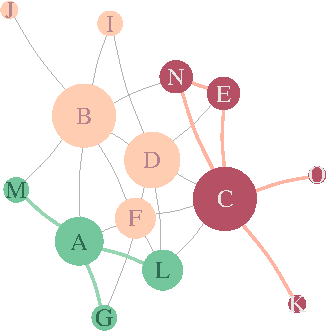
\includegraphics{NetMed_files/figure-latex/separation-1.pdf}
\caption{\label{fig:separation}Disease-Separation. A schematic of a PPI, in pink we see genes associated with a disease A, and in green genes associated to disease B.}
\end{figure}

The separation of diseases A and B is given by: \[
<d_{AA}> = 1.5
\]

\[
<d_{BB}> = 1.5
\]

\[
<d_{AB}> = 2.7
\] \[
S_{AB} = 2.7 - \frac{1.5+ 1.5}2 = 1.2
\]

\hypertarget{example-in-real-data-1}{%
\subsection{Example in real data}\label{example-in-real-data-1}}

\begin{Shaded}
\begin{Highlighting}[]
\NormalTok{sab }\OtherTok{=} \FunctionTok{separation}\NormalTok{(gPPI, GDA\_Interest)}
\end{Highlighting}
\end{Shaded}

\begin{verbatim}
##   |                                                                              |                                                                      |   0%  |                                                                              |==============                                                        |  20%  |                                                                              |============================                                          |  40%  |                                                                              |==========================================                            |  60%  |                                                                              |========================================================              |  80%  |                                                                              |======================================================================| 100%
\end{verbatim}

\begin{verbatim}
## Calculating S_ab..
\end{verbatim}

\begin{verbatim}
##   |                                                                              |                                                                      |   0%  |                                                                              |==============                                                        |  20%  |                                                                              |============================                                          |  40%  |                                                                              |==========================================                            |  60%  |                                                                              |========================================================              |  80%  |                                                                              |======================================================================| 100%
\end{verbatim}

\begin{verbatim}
## Done..
\end{verbatim}

\begin{Shaded}
\begin{Highlighting}[]
\NormalTok{Sep\_ex2 }\OtherTok{=}\NormalTok{ sab}\SpecialCharTok{$}\NormalTok{Sab }\SpecialCharTok{\%\textgreater{}\%} \FunctionTok{as.matrix}\NormalTok{()}

\NormalTok{Sep\_ex2[}\FunctionTok{lower.tri}\NormalTok{(Sep\_ex2)] }\OtherTok{=} \FunctionTok{t}\NormalTok{(Sep\_ex2)[}\FunctionTok{lower.tri}\NormalTok{(Sep\_ex2)]}
\end{Highlighting}
\end{Shaded}

We can visualize the network separation of the diseases using a heatmap.

\begin{Shaded}
\begin{Highlighting}[]
\NormalTok{Sep\_ex2 }\SpecialCharTok{\%\textgreater{}\%} \FunctionTok{heatmap}\NormalTok{(., }\AttributeTok{symm =}\NormalTok{ T)}
\end{Highlighting}
\end{Shaded}

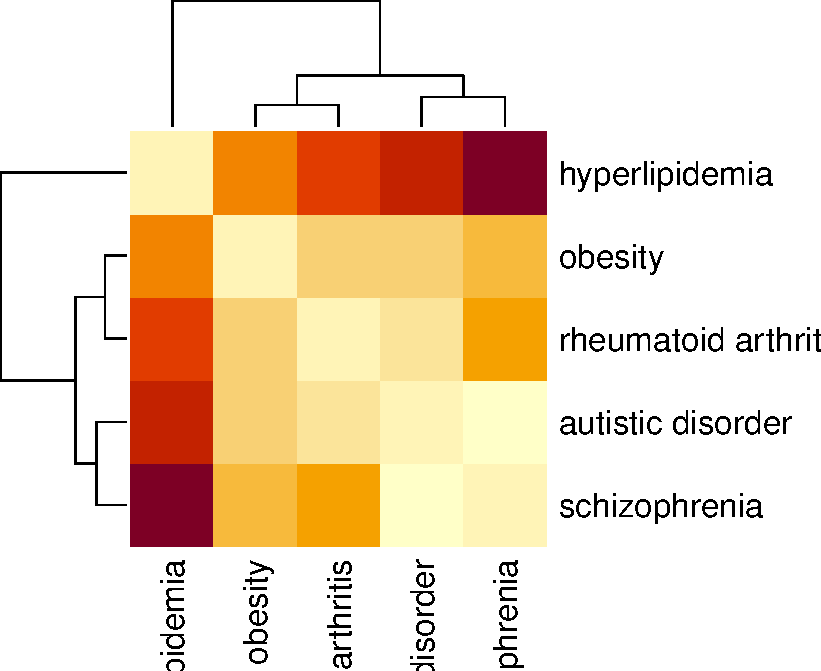
\includegraphics{NetMed_files/figure-latex/unnamed-chunk-29-1.pdf}

\hypertarget{exercises-4}{%
\section{Exercises}\label{exercises-4}}

\begin{enumerate}
\def\labelenumi{\arabic{enumi}.}
\item
  If we go back to our PPI, can we identify that the modules are indeed close or separated? Plot the network for those diseases.
\item
  Calculate the \textbf{Jaccard Index} and the \textbf{Separation} for the following diseases:

  \begin{itemize}
  \tightlist
  \item
    Schizophrenia, Bipolar Disorder, Intellectual Disability, Depressive disorder, Autistic Disorder, Unipolar Depression, Mental Depression, Major Depressive Disorder, Mood Disorders, Cocaine Dependence, Cocaine Abuse, Cocaine-Related Disorders, Substance abuse problem, Drug abuse, Drug Dependence, Drug habituation, Drug Use Disorders, Substance-Related Disorders, Psychotic Disorders, Obesity, hyperlipidemia, Rheumatoid Arthritis, Prostatic Neoplasms, Mammary Neoplasms, Mammary Neoplasms, Human Malignant neoplasm of stomach, Stomach Neoplasms, Colorectal Neoplasms, Malignant neoplasm of lung, Lung Neoplasms, Malignant neoplasm of prostate.
  \end{itemize}
\item
  Optional: Try to make the network visualization for the heatmap of \texttt{Sep\_ex2}. Use diseases as nodes, and their weight as links.
\item
  Optional: Plot the PPI with genes selected in \texttt{GDA\_Interest} where each node is a piechart representing which diseases are associated to that particular gene. Tip: Check \texttt{vertex.shape.pie} for help.
\end{enumerate}

\hypertarget{method-for-drug-repurpusing}{%
\chapter{Method for drug-repurpusing}\label{method-for-drug-repurpusing}}

In this Chapter we will learn how to calculate the proximity of a drug to a disease - and infer drug repurpusing (Session \ref{proximity})- based on network methodologies.

There are different methods that are used for drug-repurpusing based on networks, such as the \textbf{diffusion state distance (DSD)} \citep{Cao2013}, that uses a \textbf{graph diffusion property} to derive a similarity metric for pairs of nodes that takes into account how similarly they affect the rest of the network; and \textbf{AI-based methods}, where a heterogeneous graph \(G = (V,R)\) with N nodes \(v_i \in V\) representing distinct types of biomedical entities and labeled edges representing semantically distinct types of edges between the entities (i.e., protein-protein interactions, drug-target associations, disease-protein associations, and drug-disease indications) and are tasked to predict drugs for a particular disease \citep{Zitnik2018}. Due to the limited time, we will focus only on the proximity based method.

For this, we will be using the \texttt{R} package \texttt{NetSci} and to make the appropriate visualizations we will use \texttt{igraph}.

\hypertarget{proximity}{%
\section{Proximity}\label{proximity}}

Given G, the set of Disease-Genes, T, the set of drug targets, and d(g,t), the shortest path length between nodes \(g \in G\) and \(t \in T\) in the network, the proximity can be defined as \citep{Guney2016}:

\[ 
d(g,t)  = \frac{1}{|\left|T\right||}\sum_{t\in T}\underset{v\in V}\min{d(g,t)}
\]

A visual representation of the method can be seen in Figure \ref{fig:proximity}.

The proximity for drug 2 to the disease is calculated by the average of the shortest path from its targets to the disease genes. The shortest path from N to D is 1, from F to D is 3, the average is 2.

For Drug 1 we have: \[d(Drug_1, disease) = \frac{2 + 2 + 1}{3} = 1.66\]

\begin{figure}
\centering
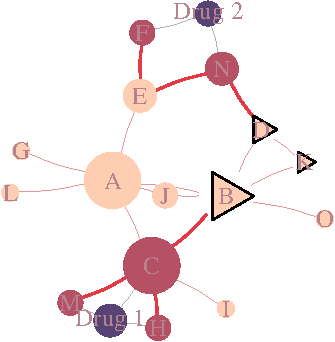
\includegraphics{NetMed_files/figure-latex/proximity-1.pdf}
\caption{\label{fig:proximity}Drug-Target \& Disease-Module Proximity. Triangles represents Disease Associated Genes, while circles represent non-associated genes. In dark purple, we see the drugs and light purple, its targets.}
\end{figure}

Similarly to the LCC (\ref{diseasemodule}) it is important to calculate a measure of randomness associate to the proximity. In the same sense, it is important that the nodes being randomized, they are not simply randomly selected from the pool of proteins in the PPI, but rather selected from matching degree proteins. To calculate the significance of the proximity one can calculate its Z-Score or simply calculate the empirical probability under the curve from the empirical distribution. Similartly as before, the Z-score is given by:

\[
Z-Score_{d(g,t)} = \frac{d(g,t) - \mu_{d(g,t)}}{\sigma_{d(g,t)}}
\]

\hypertarget{example-in-real-data-2}{%
\section{Example in real data}\label{example-in-real-data-2}}

Let's try it to identify drugs that could work for our disease sets. Let's focus on hyperlipidemia and focus on 5 drugs at first.

\begin{itemize}
\tightlist
\item
  Asenapine,
\item
  Phentermine,
\item
  Simvastatin,
\item
  Pizotifen,
\item
  Eprotirome.
\end{itemize}

\begin{Shaded}
\begin{Highlighting}[]
\NormalTok{hyperlipidemia\_genes }\OtherTok{=}\NormalTok{ Cleaned\_GDA }\SpecialCharTok{\%\textgreater{}\%} \FunctionTok{filter}\NormalTok{(diseaseName }\SpecialCharTok{==} \StringTok{\textquotesingle{}hyperlipidemia\textquotesingle{}}\NormalTok{) }\SpecialCharTok{\%\textgreater{}\%} \FunctionTok{pull}\NormalTok{(geneSymbol) }\SpecialCharTok{\%\textgreater{}\%} \FunctionTok{unique}\NormalTok{()}

\NormalTok{Asenapine\_t }\OtherTok{=}\NormalTok{ DT }\SpecialCharTok{\%\textgreater{}\%} 
  \FunctionTok{filter}\NormalTok{(Name }\SpecialCharTok{==} \StringTok{\textquotesingle{}Asenapine\textquotesingle{}}\NormalTok{) }\SpecialCharTok{\%\textgreater{}\%}
  \FunctionTok{pull}\NormalTok{(Gene\_Target)}

\NormalTok{Asenapine\_t}
\end{Highlighting}
\end{Shaded}

\begin{verbatim}
##  [1] "HTR1A"  "HTR1B"  "HTR2A"  "HTR2B"  "HTR2C"  "HTR5A"  "HTR6"   "HTR7"  
##  [9] "DRD2"   "DRD3"   "DRD4"   "DRD1"   "ADRA1A" "ADRA2A" "ADRA2B" "ADRA2C"
## [17] "HRH1"   "HRH2"   "ADRB1"  "ADRB2"  "UGT1A4" "CYP1A2" "CYP2D6" "CYP3A4"
## [25] "ALB"    "ORM1"
\end{verbatim}

\begin{Shaded}
\begin{Highlighting}[]
\FunctionTok{proximity\_average}\NormalTok{(gPPI, }
                  \AttributeTok{source =}\NormalTok{ hyperlipidemia\_genes, }
                  \AttributeTok{targets =}\NormalTok{ Asenapine\_t)}
\end{Highlighting}
\end{Shaded}

\begin{verbatim}
## [1] 1.961538
\end{verbatim}

Let's do it in a loop:

\begin{Shaded}
\begin{Highlighting}[]
\NormalTok{drugs }\OtherTok{=} \FunctionTok{c}\NormalTok{(}\StringTok{"Asenapine"}\NormalTok{, }
          \StringTok{\textquotesingle{}Phentermine\textquotesingle{}}\NormalTok{, }
          \StringTok{\textquotesingle{}Simvastatin\textquotesingle{}}\NormalTok{, }
          \StringTok{\textquotesingle{}Pizotifen\textquotesingle{}}\NormalTok{,}
          \StringTok{\textquotesingle{}Eprotirome\textquotesingle{}}\NormalTok{)}

\NormalTok{p }\OtherTok{=} \FunctionTok{list}\NormalTok{()}
\ControlFlowTok{for}\NormalTok{(i }\ControlFlowTok{in} \DecValTok{1}\SpecialCharTok{:}\FunctionTok{length}\NormalTok{(drugs))\{}
\NormalTok{  d }\OtherTok{=}\NormalTok{ drugs[i]}
\NormalTok{  Drug\_targets }\OtherTok{=}\NormalTok{ DT }\SpecialCharTok{\%\textgreater{}\%} 
    \FunctionTok{filter}\NormalTok{(Name }\SpecialCharTok{\%in\%}\NormalTok{ d) }\SpecialCharTok{\%\textgreater{}\%}
    \FunctionTok{pull}\NormalTok{(Gene\_Target)}
  
\NormalTok{  prox }\OtherTok{=} \FunctionTok{proximity\_average}\NormalTok{(gPPI, }
                           \AttributeTok{source =}\NormalTok{ hyperlipidemia\_genes, }
                           \AttributeTok{targets =}\NormalTok{ Drug\_targets)}
  
\NormalTok{  p[[i]] }\OtherTok{=} \FunctionTok{data.frame}\NormalTok{(}\AttributeTok{prox =}\NormalTok{ prox, }
                      \AttributeTok{ntargets =} \FunctionTok{length}\NormalTok{(Drug\_targets), }
                      \AttributeTok{drug =}\NormalTok{ d)}
\NormalTok{\}}

\NormalTok{p }\SpecialCharTok{\%\textless{}\textgreater{}\%} \FunctionTok{bind\_rows}\NormalTok{()}
\end{Highlighting}
\end{Shaded}

Now, let's do the same, but also calculating the significance of the proximity.

\begin{Shaded}
\begin{Highlighting}[]
\NormalTok{Drug\_Target }\OtherTok{=}\NormalTok{ DT }\SpecialCharTok{\%\textgreater{}\%} 
  \FunctionTok{filter}\NormalTok{(Name }\SpecialCharTok{\%in\%}\NormalTok{ drugs) }\SpecialCharTok{\%\textgreater{}\%} 
  \FunctionTok{select}\NormalTok{(Name, Gene\_Target) }\SpecialCharTok{\%\textgreater{}\%} 
  \FunctionTok{unique}\NormalTok{()}

\FunctionTok{names}\NormalTok{(Drug\_Target) }\OtherTok{=} \FunctionTok{c}\NormalTok{(}\StringTok{\textquotesingle{}ID\textquotesingle{}}\NormalTok{, }\StringTok{"Target"}\NormalTok{ )}

\NormalTok{proximity\_significance }\OtherTok{=} \FunctionTok{avr\_proximity\_multiple\_target\_sets}\NormalTok{(}
  \AttributeTok{set =}\NormalTok{ drugs,}
  \AttributeTok{G =}\NormalTok{ gPPI,}
  \AttributeTok{ST =}\NormalTok{ Drug\_Target,}
  \AttributeTok{source =}\NormalTok{ hyperlipidemia\_genes,}
  \AttributeTok{N =} \DecValTok{10}\NormalTok{,}
  \AttributeTok{bins =} \DecValTok{100}\NormalTok{,}
  \AttributeTok{min\_per\_bin =} \DecValTok{20}
\NormalTok{)}
\end{Highlighting}
\end{Shaded}

\begin{verbatim}
##   |                                                                              |                                                                      |   0%  |                                                                              |==============                                                        |  20%  |                                                                              |============================                                          |  40%  |                                                                              |==========================================                            |  60%  |                                                                              |========================================================              |  80%  |                                                                              |======================================================================| 100%
\end{verbatim}

Which are the drugs that we can use for hyperlipidemia?

\begin{Shaded}
\begin{Highlighting}[]
\NormalTok{proximity\_significance}
\end{Highlighting}
\end{Shaded}

\begin{verbatim}
##                    Drug targets targets_G proximity  IC_97.5   IC_2.5 p_gt p_lt
## Asenapine     Asenapine      26        26  1.961538 2.251923 1.978846  0.9  0.1
## Phentermine Phentermine       7         7  2.000000 2.792857 2.142857  1.0  0.0
## Simvastatin Simvastatin      20        19  2.157895 2.619737 2.327632  1.0  0.0
## Pizotifen     Pizotifen      17        17  2.058824 2.294118 1.876471  0.7  0.3
## Eprotirome   Eprotirome       2         2  1.500000 2.000000 2.000000  1.0  0.0
##                      Z
## Asenapine   -1.7084389
## Phentermine -1.8973666
## Simvastatin -2.8460499
## Pizotifen   -0.5217939
## Eprotirome        -Inf
\end{verbatim}

Now, let us check those drug indications:

\begin{Shaded}
\begin{Highlighting}[]
\NormalTok{Indication }\OtherTok{=}\NormalTok{ DT }\SpecialCharTok{\%\textgreater{}\%} 
  \FunctionTok{filter}\NormalTok{(Name }\SpecialCharTok{\%in\%}\NormalTok{ drugs) }\SpecialCharTok{\%\textgreater{}\%} 
  \FunctionTok{select}\NormalTok{(Name, Indication) }\SpecialCharTok{\%\textgreater{}\%} 
  \FunctionTok{unique}\NormalTok{()}

\NormalTok{Indication}
\end{Highlighting}
\end{Shaded}

\begin{verbatim}
##           Name
## 1: Phentermine
## 2: Simvastatin
## 3:  Eprotirome
## 4:   Pizotifen
## 5:   Asenapine
##                                                                                                                                                                                                                                                                                                                                                                                                                                                                                                                                                                                                                                                                                                                                                                                                                                                                                                                                                                                                                                                                                                                                                                                                                                                                                                                                                                                                                                                                                                                                                                                                                                                                                                                                                                                                                     Indication
## 1:                                                                                                                                                                                                                                                                                                                                                                                                                                                                                                                                                                                                                                                                                                                                                                                                                                                                                                                                 Phentermine is indicated, alone or in combination with topiramate, as a short-term adjunct, not pass a few weeks, in a regimen of weight reduction based on exercise, behavioral modifications and caloric restriction in the management of exogenous obesity for patients with an initial body mass index (BMI) greater than 30 kg/m2 or greater than 27 kg/m2 in presence of other risk factors such as controller hypertension, diabetes or hyperlipidemia.[FDA label]\r\n\r\nExogenous obesity is considered when the overweight is caused by consuming more food than the person activity level warrants. This condition commonly causes an increase in fat storage. It is an epidemic condition in the United States where over two-thirds of adults are overweight or obese and one in three Americans is obese. In the world, the incidence of obesity has nearly doubled.[A174391]
## 2: Simvastatin is indicated for the treatment of hyperlipidemia to reduce elevated total cholesterol (total-C), low-density lipoprotein cholesterol (LDL‑C), apolipoprotein B (Apo B), and triglycerides (TG), and to increase high-density lipoprotein cholesterol (HDL-C).[F4655, F4658]\r\n\r\nThis includes the treatment of primary hyperlipidemia (Fredrickson type IIa, heterozygous familial and nonfamilial), mixed dyslipidemia (Fredrickson type IIb), hypertriglyceridemia (Fredrickson type IV hyperlipidemia), primary dysbetalipoproteinemia (Fredrickson type III hyperlipidemia), homozygous familial hypercholesterolemia (HoFH) as an adjunct to other lipid-lowering treatments, as well as adolescent patients with Heterozygous Familial Hypercholesterolemia (HeFH).[F4655, F4658]\r\n\r\nSimvastatin is also indicated to reduce the risk of cardiovascular morbidity and mortality including myocardial infarction, stroke, and the need for revascularization procedures. It is primarily used in patients at high risk of coronary events because of existing coronary heart disease, diabetes, peripheral vessel disease, history of stroke or other cerebrovascular disease.[F4655, F4658]\r\n\r\nPrescribing of statin medications is considered standard practice following any cardiovascular events and for people with a moderate to high risk of development of CVD. Statin-indicated conditions include diabetes mellitus, clinical atherosclerosis (including myocardial infarction, acute coronary syndromes, stable angina, documented coronary artery disease, stroke, trans ischemic attack (TIA), documented carotid disease, peripheral artery disease, and claudication), abdominal aortic aneurysm, chronic kidney disease, and severely elevated LDL-C levels.[A181087, A181406]
## 3:                                                                                                                                                                                                                                                                                                                                                                                                                                                                                                                                                                                                                                                                                                                                                                                                                                                                                                                                                                                                                                                                                                                                                                                                                                                                                                                                                                                                                                                                                                                                                                                                                                                                                                                                           Investigated for use/treatment in hyperlipidemia, metabolic disease, and obesity.
## 4:                                                                                                                                                                                                                                                                                                                                                                                                                                                                                                                                                                                                                                                                                                                                                                                                                                                                                                                                                                                                                                                                                                                                                                                                                                                                                                                                                                                                                                                                                                                                                                                                                                                                                                                                                             Indicated for the prophylactic management of migraines [L2292].
## 5:                                                                                                                                                                                                                                                                                                                                                                                                                                                                                                                                                                                                                                                                                                                                                                                                                                                                                                                                                                                                                                                                                                                                                                                                                                                                                                                                                                                                                                                                                                                                                                                                                                                                      Used for treatment in psychosis, schizophrenia and schizoaffective disorders, manic disorders, and bipolar disorders as monotherapy or in combination.
\end{verbatim}

\hypertarget{exercises-5}{%
\section{Exercises}\label{exercises-5}}

\begin{enumerate}
\def\labelenumi{\arabic{enumi}.}
\item
  Test the same drugs for all the 5 other diseases we are interested in. How those values compare?

  \begin{itemize}
  \tightlist
  \item
    Autistic Disorder;
  \item
    Obesity;
  \item
    Hyperlipidemia;
  \item
    Rheumatoid Arthritis.
  \end{itemize}
\item
  Choose one disease and visualize the disease module along with each of the drugs we tested.
\end{enumerate}

\hypertarget{summary}{%
\chapter{Summary}\label{summary}}

In this course we learned how to identify disease modules, disease separation and how to repurpuse drugs using a network medicine approach.

  \bibliography{book.bib,packages.bib}

\end{document}
